\documentclass[uplatex,dvipdfmx,11pt,a4paper,openany]{bxjsbook}
\geometry{margin=24mm}
\usepackage{amsmath,amssymb,mathtools}
\usepackage[dvipdfmx]{graphicx}
\usepackage{tabularx,array}
\usepackage[dvipdfmx]{xcolor}
\usepackage{enumitem}
\usepackage[most]{tcolorbox}
\usepackage[dvipdfmx]{hyperref}
\usepackage{pxjahyper}
\hypersetup{colorlinks=true,linkcolor=blue!45!black,urlcolor=blue!55!black}
\setlist{nosep,leftmargin=2em}
\setcounter{tocdepth}{2}
\definecolor{LectureBlue}{HTML}{245A8D}
\definecolor{ColumnInk}{HTML}{563D2D}
\definecolor{ColumnPaper}{HTML}{FFF8E8}
\definecolor{NotePaper}{HTML}{F2F6FA}
\newtcolorbox{lectureblock}[1]{breakable,colback=NotePaper,colframe=LectureBlue!55,
  title={#1},boxrule=.6pt,arc=1.5mm,left=2mm,right=2mm,top=1mm,bottom=1mm}
\newtcolorbox{columnbox}[1]{breakable,enhanced,colback=ColumnPaper,colframe=orange!55!black,
  title={コラム：#1},boxrule=.9pt,arc=2mm,left=3mm,right=3mm,top=2mm,bottom=2mm,
  borderline west={3pt}{0pt}{orange!70!black}}
\newtcolorbox{detailblock}[1]{breakable,colback=white,colframe=black!30,title={#1},boxrule=.4pt}
\newenvironment{noteblock}{\begin{quote}\color{black!72}\small}{\end{quote}}
\newenvironment{leadparagraph}{\begin{quote}\large\color{ColumnInk}}{\end{quote}}
\newenvironment{figuretext}{\begin{quote}\small\color{black!65}\emph{図中の情報：}}{\end{quote}}
\newcommand{\columnheading}[1]{\par\medskip{\large\color{ColumnInk}#1}\par\smallskip}
\newcommand{\columnsubheading}[1]{\par\smallskip{\color{ColumnInk}\emph{#1}}\par\smallskip}
\title{確率論と統計学 I\\講義ノート}
\author{中島秀太}
\date{2026年度}
\begin{document}
\frontmatter
\maketitle
\tableofcontents
\mainmatter

\chapter{確率論の基礎：歴史とコイン投げ}
Lecture 01

17世紀の賭博問題から始まった確率論がどのように発展し, 現代の科学や技術を支えているのかを歴史を見ていく
                。

\section{歴史のハイライト}
確率論はパスカルとフェルマーがゲームの配当問題を議論した書簡の往復から生まれ, 次第に数学・科学の幅広い分野へと広がっていった。

17世紀

\subsection{ゲームとギャンブルから生まれた戦略思考}
パスカルやフェルマーは偶然のゲームで勝利を導くための定量的戦略を追究し, 離散確率論の枠組みを築き上げた。

\begin{noteblock}
当時のニュートン力学は決定論的であり, 確率的な視点とはまだ交わっていなかった。
\end{noteblock}

19世紀

\subsection{相転移の謎に挑んだ統計物理}
マクスウェルやボルツマンは氷・水・水蒸気の相転移を説明するため, 巨視的現象を微視的粒子の確率モデルとして捉え直した。

\begin{noteblock}
統計物理では初期条件や観測時間に不確かさを導入し, 決定論的な力学に意図的に確率を重ね合わせる。
\end{noteblock}

20世紀

\subsection{量子ゆらぎが切り開いた新たな確率論}
ボルンらによる量子力学は粒子の位置と速度を同時に確定できないことを示し, 連続的な確率モデルと公理的確率論へと発展した。

\begin{noteblock}
波動関数の確率解釈によって, 確率論は物理学の基礎概念へと飛躍する。
\end{noteblock}

\begin{itemize}
\item \emph{ブレーズ・パスカル (1623-1662)}期待値の概念と「パスカルの三角形」を発展させ, ゲームに確率の視点を導入した。
\item \emph{ピエール・ド・フェルマー (1607-1665)}賭博問題を組み合わせ論で解く方針を示し, 離散構造の解析に道を開いた。
\item \emph{ヤコブ・ベルヌーイ (1654-1705)}『推測術』で大数の法則を示し, 長期的な安定性の概念を確立した。
\item \emph{ピエール＝シモン・ラプラス (1749-1827)}確率を解析的に体系化し, ベイズ推論や天体運動への応用を推進した。
\item \emph{アンドレイ・コルモゴロフ (1903-1987)}測度論的公理系を提示し, 現代確率論の土台を築いた。
\end{itemize}

\section{確率論と他分野}
\subsection{確率と統計3>}
確率空間はモデル側と観測側をつなぐ基盤であり, 確率論と統計学がどのように往復しながら知識を更新していくのかを理解する鍵になる。

\begin{figuretext}
確率論 \quad モデルから予測へ \quad (Model → Prediction) \quad 「モデルが正しければ, このデータが観測 \quad される確率はどのくらいか？」 \quad 統計学 \quad データからモデルへ \quad (Data → Model) \quad 「観測されたデータから, \quad 最も妥当なモデルは何か？」 \quad 理論的基礎 \quad 検証と改良 \quad 実世界のデータ \quad 確率モデル
\end{figuretext}

図1: モデルとデータの往復

\begin{itemize}
\item 天気予報で示される「降水確率40\%」は, 気象データを基に構築された確率モデルによる推定値である。
\item 医療の検査精度や治療成功率は確率測度として表現され, 意思決定やリスク評価に利用される。
\item 交通渋滞の予測や公共交通機関のダイヤ設計には, 確率的な需要モデルが組み込まれている。
\item カードゲームや宝くじなどの娯楽は確率計算に基づいて設計され, フェアネスや期待値の議論に直結する。
\end{itemize}

\subsection{学際的な広がり}
\begin{figuretext}
確率論 \quad 統計学 \quad 量子力学 \quad 金融工学 \quad 機械学習 \quad 情報理論 \quad 暗号技術 \quad 遺伝学 \quad 保険数理
\end{figuretext}

図2: 確率論が結ぶ学際領域の例

\section{コイン投げで学ぶ確率空間}
\subsection{コイントスで学ぶ標本空間}
\paragraph{例}
\subsubsection{のコイン投げ}
表 (H)

裏 (T)

$\Omega = \{H, T\}$ とおき, 公平なコインなら $P(H) = P(T) = \tfrac{1}{2}$ とする。


\paragraph{例}
\subsection{2回のコイン投げ}
標本空間は $\Omega = \{(H,H), (H,T), (T,H), (T,T)\}$ となり, 各要素の確率は $\tfrac{1}{4}$。

「少なくとも1回は表」という事象 $A = \{(H,H), (H,T), (T,H)\}$ の確率は $P(A) = \tfrac{3}{4}$。


\begin{figuretext}
2回のコイントスの標本空間 Ω \quad (H, H) \quad H \quad 確率 1/4 \quad (H, T) \quad T \quad (T, H) \quad (T, T)
\end{figuretext}

図3: 2回のコイントスで得られる結果

\subsection{有限確率空間の一般形}
$\Omega$ を有限集合とし, 各 $\omega \in \Omega$ に $0$ 以上 $1$ 以下の重み $p(\omega)$ を割り当て, 総和を $1$ に正規化する。

\begin{itemize}
\item 確率測度 $P(A) = \sum_{\omega \in A} p(\omega)$ と定めると, $(\Omega, 2^{\Omega}, P)$ が有限確率空間となる。
\item 例: 三回のコイントス, 二つのサイコロ, 有限状態マルコフ連鎖など。
\end{itemize}

\begin{noteblock}
非加算的な場合, 単点集合の確率が 0 でも集合全体に正の確率を割り当てられる。
\end{noteblock}

\section{測度論的確率論の基礎}
\subsection{シグマ加法族}
集合 $\Omega$ 上の族 $\mathcal{F}$ が次の条件を満たすとき $\mathcal{F}$ をシグマ加法族と呼ぶ。

\begin{itemize}
\item $\Omega \in \mathcal{F}$
\item もし $A \in \mathcal{F}$ ならば $A^{c} \in \mathcal{F}$
\item $A_i \in \mathcal{F}$, $i \in \mathbb{N}$ ならば $\bigcup_{i=1}^{\infty} A_i \in \mathcal{F}$
\end{itemize}

集合の列$A_i$について、$A_i\cap A_j=\emptyset\quad (i\neq j)$であるとき、互いに素であると呼ぶ。

\subsection{確率測度の定義}
集合 $\Omega$ 上のシグマ加法族 $\mathcal{F}$ に対して, 写像 $P : \mathcal{F} \to [0,1]$ が次の三条件を満たすとき, $P$ を確率測度と呼ぶ。

\begin{itemize}
\item $P(A) \ge 0$ （非負性）
\item $P(\Omega) = 1$ （全体の確率は1）
\item 互いに素な $A_i \in \mathcal{F}$ に対して $P\!\left(\bigcup_{i=1}^{\infty} A_i\right) = \sum_{i=1}^{\infty} P(A_i)$ （可算加法性）
\end{itemize}

\paragraph{補足}
確率測度は測度論の枠組みに基づくものであり, その定義はルベーグ測度の拡張と対応している。したがって確率空間 $(\Omega, \mathcal{F}, P)$ は, 測度空間の特別な場合とみなせる。


\paragraph{補足}
$\mathbb{R}^d$ のボレルシグマ代数は開集合族から生成され, 連続モデルの標準的な選択となる。


確率空間は三つ組 $(\Omega, \mathcal{F}, P)$ であり, 測度 $P$ は $\mathcal{F}$ 上の可算加法的な写像となる。

\subsection{確率空間の基本性質}
公理から直ちに導かれる性質を整理する。

\begin{itemize}
\item $P(A^{c}) = 1 - P(A)$
\item $A \subseteq B$ ならば $P(A) \le P(B)$
\item $P(A \cup B) = P(A) + P(B) - P(A \cap B)$
\item $P\bigl(\bigcup_{i=1}^{\infty} A_i\bigr) \le \sum_{i=1}^{\infty} P(A_i)$（可算劣加法性）
\end{itemize}

\paragraph{補足}
包含排除の公式は有限個の事象にも拡張され, 交差部分の情報を補正項として扱う。


\paragraph{定義}
\subsection{定義（単調増加列）}
可測集合列 $(A_n)_{n\ge 1}$ が \emph{単調増加} であるとは, すべての $n$ に対して $A_n \subseteq A_{n+1}$ が成り立つことをいう。このとき $A_n$ が極限に向かって「広がっていく」ので $(A_n)$ を増加列とも呼ぶ。


\paragraph{定理}
\subsection{定理（単調増加列に対する連続性）}
測度空間 $(\Omega, \mathcal{F}, P)$ 上の可測集合列 $(A_n)_{n\ge 1}$ が単調増加であるとする。$A = \bigcup_{n=1}^{\infty} A_n$ とおくと, 次が成り立つ。

\[\lim_{n\to\infty} P(A_n) = P\!\left(\bigcup_{n=1}^{\infty} A_n\right).\]

\paragraph{証明}
\emph{証明.}

$C_1 = A_1$, $C_n = A_n \setminus A_{n-1}$（$n\ge 2$）と定めると, $C_n$ は互いに素で $A_m = \bigcup_{k=1}^{m} C_k$, $A = \bigcup_{k=1}^{\infty} C_k$ となる。

可算加法性より $P(A_m) = \sum_{k=1}^{m} P(C_k)$, $P(A) = \sum_{k=1}^{\infty} P(C_k)$。右辺は非負項の級数なので部分和の極限が全和に一致し, $\lim_{m\to\infty} P(A_m) = P(A)$ が従う。$\square$



\section{レポート課題}
講義内容を踏まえ, 以下の問いについてレポートとしてまとめてください。必要に応じて参考文献や図表を添付し, 根拠を明確に示しましょう。

\begin{enumerate}
\item 歴史の中で興味を持った出来事または人物を一つ選び, 当時の背景や影響を深掘りせよ。
\item $[0, 1]$ 内のすべての部分集合に確率が定義できると仮定したときに生じる問題点を議論せよ。
\item 単調増加列に対する連続性を用いて、可算劣加法性を示せ: \[P\bigl(\bigcup_{i=1}^{\infty} A_i\bigr) \le \sum_{i=1}^{\infty} P(A_i)\]
\end{enumerate}

© 2025 確率論講義 - すべての権利を留保します


\clearpage
\begin{columnbox}{確率は「数え上げ」から、「$\sigma$-加法族」へ}
\begin{leadparagraph}
大学の確率論で最初に触れるのは、面積（あるいは長さ・体積）で確率をとらえる考え方だ。事象を集合として描けば、面積が大きいほど「起こりやすい」と感じられる。学びを進めると、次に立ちはだかる壁は、なぜ確率空間に $\sigma$ 加法族が現れるのかという点。ここでは、その道筋をやわらかく整理しておきたい。
\end{leadparagraph}

\columnheading{等確率の原理：数え上げから始まる}
中学で扱う確率は数え上げから始まる。より正確には、事象 $A$ の確率は

\[\mathbb P(A)=\frac{\text{Aの数}}{\text{全体の数}}\tag{★}\]

で与えられる。結局のところ、全体の数と $A$ の数を数える作業に帰着する。例えば、表と裏が同確率 $1/2$ のコインを2回投げ、表の数がちょうど1回になる確率では、全体 $4$ 通り、該当が $2$ 通りとなり、確率は $2/4=1/2$ になる。

\begin{noteblock}
公式（★）は、各「単事象」が同じ確率で現れるという等確率の原理を前提にしている点を押さえておきたい。
\end{noteblock}

\columnheading{非等確率への拡張：足し合わせに移る}
単事象の起こりやすさが異なる場合、確率は構成する単事象の確率を足し合わせて求めることになる。例えば、表の確率が $1/4$、裏が $3/4$ のコインを2回投げ、表がちょうど1回となる確率は次のように求める:

\[\mathbb P(\text{表裏})=\tfrac{1}{4}\cdot\tfrac{3}{4}=\tfrac{3}{16},\quad
        \mathbb P(\text{裏表})=\tfrac{3}{4}\cdot\tfrac{1}{4}=\tfrac{3}{16},\]
\[\Rightarrow\ \mathbb P(\text{表がちょうど1回})=\tfrac{3}{16}+\tfrac{3}{16}=\tfrac{3}{8}.\]

先の公式（★）は、単事象がすべて $1/(\text{全体の数})$ の確率で現れるという仮定のもとでの特別な姿にすぎない。非等確率では「数え上げ」から「足し合わせ」へ視点が移る。

\columnheading{無限集合の壁：「数え上げ」をそのままには使えない}
無限集合の世界へ、概念を広げたくなるのは自然である。たとえば $[0,1]$ から一様に点を選ぶ操作を、数学的にきちんと表したくなる。しかし全体が非可算になると、素朴な足し算は行き詰まる。実際次のような定理が成り立つ:

定理

正値列 $(a_i)_{i\in I}$ が
          \[\sup_{F\subset I\ \text{有限}}\sum_{i\in F} a_i < \infty\]
          を満たすなら、$I$ は可算である。

\begin{noteblock}
したがって $\sum_{i\in \Omega} p_i = 1$ を仮定した瞬間に、$\{i:\,p_i>0\}$ は可算になり、非可算な「全体」を単純な重み付きの和で考えることは不可能となる。
\end{noteblock}

\columnheading{コルモゴロフの視点：和から積分へ}
非可算な全体の上で確率を考えるときに重要になるのは、和 $\sum$ を積分 $\int$ に置き換えるという考え方である。たとえば $[0,1]$ 上で一様に点をとるモデルを考えると、区間 $[a,b]$ にその点が含まれる確率は長さ $|b-a|$ と定めるのが自然である。このとき
\[
|b-a| = \int_{0}^{1} \mathbf{1}\{x \in [a,b]\}\, dx
\]
のように、確率が指示関数の積分として表現される。ここで $\mathbf{1}\{A\}$ は事象 $A$ が起これば $1$、そうでなければ $0$ を返す関数である。この発想を一般化し、確率論に統一的な枠組みを与えたのがコルモゴロフである。コルモゴロフは、さらに可算と非可算を同時に扱うため、ルベーグ測度論を採用するに至った。たとえば

\[P(A)=\tfrac{1}{2}\,\mathbf{1}_{\{0\in A\}}+\tfrac{1}{2}\,\lambda(A\cap[0,1])\]

のように、点 $0$ の原子と $[0,1]$ 上の一様分布（ルベーグ測度 $\lambda$）を組み合わせた確率を素直に定義できる。鍵は、面積をあらゆる集合で測ろうとせず、性質の良い集合族――ボレル可測集合――に対象を絞ることである。

\columnheading{なぜ一般の $\sigma$ 加法族か：情報という見方}
確率論では「情報」という視点が重要になる。たとえば毎日の天気を考えると、今日までの天気は知っているが、明日以降はまだ知らないと捉えるのが自然だ。このとき、今日までの天気で条件づけたときの、明日の天気が晴れである確率を計算するといった問題が考えられる。つまり、今日までに得た''情報"をどのような数学的対象として記述するかが課題になる。

コルモゴロフの革新的なアイデアは、情報を $\sigma$ 加法族で表すという発想にある。より具体的には、ある時刻$t$で知ることのできる事象の集まりを、その時刻の $\sigma$ 加法族 $\mathcal F_t$ に対応させる。

例としてコイン投げを二回行うモデル（時刻 $1$ に一回目、時刻 $2$ に二回目）を考える。標本空間は

\[\Omega=\{(H,H),(H,T),(T,H),(T,T)\}\]

とおく。時刻 $0$ では何も観測していないので、情報は自明な

\[\mathcal F_0=\{\emptyset,\Omega\}\]

になる。時刻 $1$ では一回目の結果だけが分かる。$A_H=\{(H,H),(H,T)\}$（一回目が表）、$A_T=\{(T,H),(T,T)\}$（一回目が裏）として、

\[\mathcal F_1=\{\emptyset,\Omega,A_H,A_T\}\]

となる。これは「一回目の結果で区別できる事象の全体」を表す。時刻 $2$ になると二回分の結果がそろうため、情報は

\[\mathcal F_2=2^{\Omega}=\{A: A\subset \Omega\}\]

に一致する。このようにして $ \mathcal F_0\subset \mathcal F_1\subset \mathcal F_2 $ という$\sigma$加法族の列が得られ、時間とともに情報が増えていくという直観に沿っている。理解には少し時間を要するが、条件付き確率の議論の中で改めて掘り下げる予定である。

\columnheading{まとめ}
短い説明で測度論の必要性を納得するのは難しいと思う。それでも、そこには明確な理由があり、現代の確率を形づくるうえで欠かせないことは覚えておいてほしい。より詳しい説明は条件付き確率の際にすることにする。

\begin{noteblock}
注）本文中の $\lambda$ はルベーグ測度。定義域はボレル可測集合族。
\end{noteblock}

\end{columnbox}

\chapter{確率論と統計学I　レジュメ2}
Lecture 2

有限な確率空間の構成と基礎的な確率変数の扱いを、コイントスの具体例を通して整理する。

\section{コイントス}
コインを2回投げる状況を考えると、結果の組み合わせ全体は次の集合で表される。

\begin{itemize}
\item (全事象) $\Omega=\{(\text{表,表}),(\text{表,裏}),(\text{裏,表}),(\text{裏,裏})\}$
\item (確率測度) $\mathbb{P}(\text{表,表})=\mathbb{P}(\text{表,裏})=\mathbb{P}(\text{裏,表})=\mathbb{P}(\text{裏,裏})=1/4$
\end{itemize}

$X$を2回投げたコインの表の数とすると、$X$は$\Omega$から$\mathbb{R}$への写像として表現できる。

$X(\text{表,表})=2,\; X(\text{表,裏})=1,\; X(\text{裏,表})=1,\; X(\text{裏,裏})=0$

このとき、分布関数は$P(X\leq a)$で定義され、次のようになる。
            \[F_X(a)=\begin{cases}
            0 & a < 0\\
            1/4 & 0 \leq  a < 1\\
            3/4 & 1 \leq a < 2\\
            1 & a \geq 2\end{cases}\]

\subsection{コイントスの視覚化}
表表

$X = 2$

$\mathbb{P} = \frac{1}{4}$

表裏

$X = 1$

$\mathbb{P} = \frac{1}{4}$

裏表

$X = 1$

$\mathbb{P} = \frac{1}{4}$

裏裏

$X = 0$

$\mathbb{P} = \frac{1}{4}$

確率空間 $(\Omega, \mathbb{P})$

(表,表)

(表,裏)

(裏,表)

(裏,裏)

$X$


$2$

$1$

$0$

0

1

2

∞

1

1/2

0
$x$
$F_X(x)$









分布関数:
$F_X(x) = \mathbb{P}(X \leq x)$
$F_X(x) = 0, 0 \leq x < 1$
$F_X(x) = 1/2, 1 \leq x < 2$
$F_X(x) = 1, x \geq 2$

\paragraph{定義}
\subsection{有限確率空間での確率変数}
有限集合$\Omega$と各元$\omega\in\Omega$に対して割り当てられた確率$p_\omega\ge 0$（$\sum_{\omega\in\Omega}p_\omega=1$）からなる有限確率空間$(\Omega,(p_\omega)_{\omega\in\Omega})$を考える。

この場合には一般の写像$X:\Omega\to\mathbb{R}$を\emph{確率変数}と呼ぶ。

\emph{分布}は各$x\in\mathbb{R}$について

\[\mathbb{P}(X=x)=\sum_{\omega\in\Omega,\; X(\omega)=x} p_\omega\]

で与えられ、\emph{分布関数}$F_X$は

\[F_X(a)=\mathbb{P}(X\le a)=\sum_{\omega\in\Omega,\; X(\omega)\le a} p_\omega\qquad(a\in\mathbb{R})\]

と定める。また\emph{期待値}は

\[\mathbb{E}[X]=\sum_{\omega\in\Omega} X(\omega)\,p_\omega\]

と定義される。


\paragraph{定義}
\subsection{一般の確率空間での定義}
\emph{確率空間}は、集合$\Omega$、$\sigma$加法族$\mathcal{F}\subset 2^\Omega$、測度$\mathbb{P}:\mathcal{F}\to[0,1]$で、$\mathbb{P}(\Omega)=1$を満たす組$(\Omega,\mathcal{F},\mathbb{P})$である。

$(\Omega,\mathcal F)$から$(\mathbb R,\mathcal B)$の可測な写像、つまり次を満たす、

$\forall A\in\mathcal{B}(\mathbb{R})\quad X^{-1}(A)=\{\omega\in\Omega: X(\omega)\in A\}\in\mathcal{F},$

とき、$X$を\emph{確率変数}と呼ぶ

同値な条件として、すべての$a\in\mathbb{R}$について$\{\omega: a\le X(\omega)\le b\}=X^{-1}([a,b])\in\mathcal{F}$でもよい。

\emph{分布（押し出し測度）}$\mu_X$は

\[\mu_X(A):=\mathbb{P}(X\in A)=\mathbb{P}(X^{-1}(A))\qquad(A\in\mathcal{B}(\mathbb{R}))\]

で定義される$\mathbb{R}$上の確率測度である。$\mu_X$のことを$X$の分布と呼ぶこともある。\emph{分布関数}$F_X:\mathbb{R}\to[0,1]$は

\[F_X(a):=\mathbb{P}(X\le a)\qquad(a\in\mathbb{R})\]

で定義され、非減少・右連続、$\lim_{a\to-\infty}F_X(a)=0$、$\lim_{a\to\infty}F_X(a)=1$を満たす。


\paragraph{例}
\subsection{記法についての注意}
\[\mathbb{P}(X \in A) = \mathbb{P}(\{\omega \in \Omega : X(\omega) \in A\}),\]
\[\mathbb{P}(X \le x) = \mathbb{P}(\{\omega : X(\omega)\le x\}),\]
\[\mathbb{P}(X = x)=\mathbb{P}(\{\omega: X(\omega)=x\}).\]


\section{例題}
\paragraph{例}
\subsection{演習問題}
次の設定の下で確率空間を定義し、確率を求めよ。

\begin{itemize}
\item $[0,1]$からの一様に点をとる操作をモデル化せよ。
\item $X(\omega)=2\omega+1$とする。$P(X\leq 1/2)$を求めよ 。
\end{itemize}


\section{レポート課題}
以下の問いについてレポートとしてまとめよ。（例えば、関連するより簡単な問題を証明するや、シミュレーションで確かめるなど、また応用例を調べるなどでも良い）必要に応じて参考文献や図表を添付し, 根拠を明確に示せ。

\begin{enumerate}
\item Feigeの予想(期待値$1$である独立な非負値確率変数の列$(X_i)$に対し, $\mathbb{P}\Big(\sum^n_{i=1} X_i \leq n+1\Big)\geq 1/e$)に関し、考察せよ。
\end{enumerate}

© 2025 確率論講義 - すべての権利を留保する


\clearpage
\begin{columnbox}{確率変数を「写像」として捉える理由}
\begin{leadparagraph}
大学３年生で初めて学んだ公理的確率論で、確率変数を「写像で定義する」と聞いたとき、正直に言えば少し奇妙に感じた。実際、入門的な本では分布 $P(X=a)$ を直接与える方式が多く、写像の話は曖昧に済まされがちだ。さらに、そもそも写像の概念は確率とは無関係である。ここでは、確率変数を写像として定義する妥当性を説明することにする。
\end{leadparagraph}

\columnheading{観測としての「写像」}
日常語では「ランダムに数をとること」が確率変数だと教わる。サイコロを１回振るモデルなら、標本空間は $\Omega=\{1,\dots,6\}$ としてよく、各元が目の値に対応する。この段階では確かに写像を持ち出さなくても困らない。

しかし２回振るなら $\Omega=\{1,\dots,6\}^2$ とするのが自然だ。このとき「１回目の目」はどう表すのがよいか。元 $(a,b)$ が観測されたとき、欲しいのは「$a$ を返す操作」だ。つまり

$X_1(\omega_1,\omega_2)=\omega_1.$

ここで大切なのは、「確率的に選ぶ」部分（$\Omega$ 上の元を選ぶ）と、「観測値を取り出す」部分（$\Omega$ から実数への写像）を分けることだ。確率変数は後者そのものとして定義する。

\columnheading{なぜ元ではなく写像なのか}
確率変数を写像として定義することには、いくつかの利点がある。

\begin{itemize}
\item $X,Y$ が写像なら、四則演算: $X+Y,\,X\cdot Y,\,g(X)$（$g$ は可測関数）も自然に定義できる。
\item $X:\Omega\to \mathbb{R}$ と確率測度 $P$ があれば、$X$ の分布は $\mu_X(A):=P(X\in A)$ と一行で定義できる。
\item さらに可測性を通じて、「その時点で見えている情報だけで定義された確率変数か」を形式的に判断できる。例えば、前回の情報列の例でいうと、$X(a,b)=1\{b=\text{表}\}$は$\mathcal{F}_1$可測でない (実際$X^{-1}(1)=\{(\text{表,表}),(\text{裏,表})\}\notin \mathcal{F}_1$) ので、時刻$1$で見えない情報を含んでいるとわかる。
\end{itemize}

上記のような利点はあるものの、正直に言えば、私はいまでもコルモゴロフがなぜ確率変数を「写像」として定義したのかを完全に理解できているわけではない。自分では到底思いつかなかった発想だと思う。しかし使い続けていくうちに、その設計の深さと便利さを少しずつ実感するようになった。天才の仕事というのは、時を経てようやくその意図の一端に触れられるものなのだろうか。

\columnheading{おわりに}
初学者には遠回りに見えるかもしれないが、複雑な確率過程や条件付き期待に踏み込むほど、この定義の美しさと力強さがはっきりと見えてくる。

\begin{noteblock}
参考：コルモゴロフ『確率論の基礎概念』(1933)
\end{noteblock}

\end{columnbox}

\chapter{期待値と極限定理}
Lecture 03

有限確率から一般の期待値の定義，分布による表現と基本性質を確認する。

\section{有限確率空間の期待値}
\paragraph{定義}
\subsection{定義（有限確率空間と確率変数）}
$\Omega$ を有限集合，$p_\omega\ge0$（$\sum_{\omega\in\Omega} p_\omega=1$）を各点の確率とする。任意の写像 $X\colon \Omega\to\mathbb{R}$ を確率変数と呼ぶ。


\paragraph{定義}
\subsection{定義（期待値）}
\[\mathbb{E}[X]=\sum_{\omega\in\Omega} X(\omega)\,p_\omega.\]


\paragraph{定理}
\subsection{基本性質}
\begin{itemize}
\item \emph{線形性}：$\mathbb{E}[X+Y]=\mathbb{E}[X]+\mathbb{E}[Y]$，$\;\mathbb{E}[\alpha X]=\alpha\,\mathbb{E}[X]$。
\item \emph{値域による表現}：$I_X:=\{x\in\mathbb{R}\mid P(X=x)>0\}$ とすると $\displaystyle \mathbb{E}[X]=\sum_{x\in I_X} x\,P(X=x)$。
\end{itemize}


\section{一般の確率変数の期待値}
\paragraph{定義}
\subsection{定義（単関数とその期待値）}
$(\Omega,\mathcal F,P)$ 上の可測集合 $A_i\in\mathcal F$ と $\alpha_i\ge0$ に対し，$X=\sum_i \alpha_i\,\mathbf 1_{A_i}$ と表せるとき $X$ を\emph{単関数}という。その期待値は

\[\mathbb{E}[X]=\sum_i \alpha_i\,P(A_i).\]


\paragraph{定義}
\subsection{定義（非負可測関数の期待値）}
$X\ge0$ 可測に対し，区間分割で作る増加列

\[X_n:=\sum_{i=1}^{\infty} \frac{i-1}{2^n}\,\mathbf 1_{\{\frac{i-1}{2^n}\le X<\frac{i}{2^n}\}}\;\uparrow\; X\]

を用いて

\[\mathbb{E}[X]:=\lim_{n\to\infty}\mathbb{E}[X_n].\]


\paragraph{定理}
\subsection{特徴付け}
$X\ge0$ なら \[\mathbb{E}[X]=\sup\{\mathbb{E}[Y]\mid 0\le Y\le X,\;Y\text{ は単関数}\}.\]


\paragraph{定義}
\subsection{定義（一般の期待値）}
$X=X^+-X^-$（$X^+=X\,\mathbf 1_{\{X\ge0\}}$, $X^-=(-X)\,\mathbf 1_{\{X<0\}}$）と分解し，$\mathbb{E}[X^+],\mathbb{E}[X^-]<\infty$ なら $X$ を\emph{可積分}といい

\[\mathbb{E}[X]=\mathbb{E}[X^+]-\mathbb{E}[X^-].\]


\section{基本性質}
\subsection{性質}
\begin{itemize}
\item \emph{線形性}：可積分 $X, Y$ と $\alpha, \beta \in \mathbb{R}$ に対し $\mathbb{E}[\alpha X + \beta Y] = \alpha \mathbb{E}[X] + \beta \mathbb{E}[Y]$。
\item \emph{単調性}：$X \le Y$ が確実に成り立つとき $\mathbb{E}[X] \le \mathbb{E}[Y]$。
\item \emph{単調収束定理}（Beppo–Levi）：$0 \le X_n \uparrow X$ なら $\mathbb{E}[X_n] \uparrow \mathbb{E}[X]$。
\item \emph{優収束定理}（DCT）：$X_n \to X$ がほぼ確実, $|X_n| \le Y$ かつ $\mathbb{E}[|Y|] < \infty$ なら $\mathbb{E}[X_n] \to \mathbb{E}[X]$。
\end{itemize}

\section{分布を使った表現}
\paragraph{定理}
\subsection{定理（LOTUS／法則による計算）}
$g \colon \mathbb{R} \to \mathbb{R}$ 可測で $g(X)$ が可積分なら

\[\mathbb{E}[g(X)] = \int_{\mathbb{R}} g(x)\,\mu_X(dx).\]

ここで $\mu_X (A)= P (X\in A)$ は $X$ の分布（法則）であり，期待値は $\mu_X$ に関する Lebesgue 積分として書ける。


\section{注意とよくある落とし穴}
\subsection{注意}
\begin{itemize}
\item $\mathbb{E}[X]$ の存在には $\mathbb{E}[|X|] < \infty$ が必要。
\item 期待値の存在は分散の存在を保証しない。
\end{itemize}

\section{レポート課題}
次を確かめよ

\begin{enumerate}
\item サイコロを３回ふる。すべての目を足し合わせた確率変数の期待値を求めよ
\item 有限確率空間での期待値の定義と一般の期待値の定義が一致することを確かめよ。このとき、$\mathcal F=2^\Omega$ととることに注意
\item $X$を単関数とし, (可測)写像 $g\colon \mathbb{R}\to[0,\infty)$が$\mathbb{E}[g(X)]<\infty$を満たすとする。これに対し
                    $\displaystyle \mathbb{E}[g(X)]=\int_{\mathbb{R}} g(x)\,d\mu_X$ を確かめよ。
\end{enumerate}

© 2025 確率論講義ノート


\clearpage
\begin{columnbox}{確率変数の期待値の定義を考える}
\begin{leadparagraph}
期待値は、離散的な場合には「値 × その確率」の総和で定義される。式で書けば $E[X]=\sum_x x\,P(X=x)$となる。一見自然だが、なぜこれが“期待する値”と呼ばれるのか。本記事では、期待値に概念を深掘りすることにする。
\end{leadparagraph}

\columnheading{コイン投げの長期平均}
公平なコインを1回投げ、表なら100円、裏なら0円獲得するとする。上記の期待値の計算に基づくとこのゲームの期待値は$0\times (1/2)+100\times (1/2)=50$円となる。一回の結果は0円か100円のどちらかで、50円は出てこないのであるが、この期待値はなにをいみしているのだろうか。

意味を与えるために、この試行を繰り返すことにする。 実際$n$ 回繰り返すと、合計金額の $n$ で割った（標本）平均は50円に近づく。回数を増やすほど平均は安定し、50円に近づく。この収束が\emph{大数の法則}であり、期待値が表すのは「長期的な平均」だと言える。

42回のコイントスを体験

\begin{noteblock}
自動で42回投げるコインを眺めながら、標本平均がどのように収束していくかを確かめてみよう。
\end{noteblock}

H

T

待機中… ボタンを押すとシミュレーションが始まります。

1投目

2投目

3投目

4投目

5投目

6投目

7投目

8投目

9投目

10投目

11投目

12投目

13投目

14投目

15投目

16投目

17投目

18投目

19投目

20投目

21投目

22投目

23投目

24投目

25投目

26投目

27投目

28投目

29投目

30投目

31投目

32投目

33投目

34投目

35投目

36投目

37投目

38投目

39投目

40投目

41投目

42投目

※ 公平なコインを仮定。表が出ると100円、裏なら0円とする。

\columnheading{“期待できる値”とズレる状況}
一方で、非常に小さい確率だが大きな値をとる確率変数の場合、期待値は直感的に期待できる値と異なる。たとえば、表の確率が1兆分の1で表なら1兆円、裏なら0円もらえるというゲームを
考える。期待値は $1$ 円になるが、実際にはほとんどの試行で0円のままになる。

こうした小さな確率で極端な値（アウトライヤーなどと呼ぶ）をもつ確率変数では、中央値（半分の結果がそれ以下・以上、つまり$P(X\geq a),P(X\leq a)\geq 1/2$、となる点）のほうが現実をよく捉える。また、期待値そのものが発散して定義不能になることすらある。

\columnheading{それでも期待値を使う理由（要点だけ）}
期待値が重要である理由として、次の２点があげられる。

\begin{enumerate}
\item \emph{線形性}：確率変数の和の期待値は各平期待値の和となる。
\item \emph{計算が易しい}：足し算するだけなので計算が易しい。
\end{enumerate}

まとめ

多くの教科書では、期待値を「だいたいこのあたりの値が期待される」といった形で柔らかく導入している。しかし実際には、期待値とは「都合がよい代表値」として考えられているにすぎず、現実の結果がその値から大きく離れることも珍しくない。
むしろ現代の確率論の多くの研究では、「期待値からどれだけ、どのように離れるか」を扱うことが主題となっており、その偏りの分布や典型的な値（例えば中央値）をいかに正確に捉えるかが重要な関心となっている。

\end{columnbox}

\chapter{Kolmogorovの拡張定理}
Lecture 04

\section{可積分性と収束の準備}
\paragraph{定義}
\subsection{定義（可積分性）}
確率変数 \(X\) に対し，正部 \(X_+=\max\{X,0\}\)，負部 \(X_-=\max\{-X,0\}\) とおく。このとき
                    \(\mathbb{E}[X_+]<\infty\) かつ \(\mathbb{E}[X_-]<\infty\) であれば \(X\) を\emph{可積分}という。


\paragraph{定理}
\subsection{命題（単調収束）}
確率変数列 \(X_n:\Omega\to\mathbb{R}\) 
について、                    \((X_0)_-\) が可積分で \(X_n\uparrow X\) が成立するならば
                    \(\mathbb{E}[\lim_{n\to\infty} X_n]=\lim_{n\to\infty}\mathbb{E}[X_n]\) が成り立つ。

\paragraph{証明}
ルベーグ測度論の単調収束定理（Beppo–Levi）の特別な場合である。



\subsection{優収束定理の補足}
確率変数列\(X_n,X\)について \(X_n\to X\quad a.s.\) かつ \(|X_n|\le Y\) を満たす可積分な確率変数 \(Y\) が存在するなら
                    \(\mathbb{E}[\lim X_n]=\mathbb{E}[X]\) が従う。

\section{有限回コイントスの復習}
\paragraph{定義}
\subsection{定義（有限試行の確率空間）}
公平なコインを \(n\) 回投げるとき
                    \(\Omega=\{+1,-1\}^n\)，\(\mathcal{F}=2^\Omega\)，\(p_\omega=2^{-n}\) と定める。測度は
                    \(P(A)=\sum_{\omega\in A}p_\omega=|A|/2^n\)。


\paragraph{例}
\subsection{例（表の個数）}
第 \(i\) 回目の結果を
                    \(X_i(\omega)=\mathbf{1}_{\{\omega_i=+1\}}\) とおく。表の総数は \(S_n=\sum_{i=1}^n X_i\) であり，
                    \(\mathbb{E}[S_n]=n/2\)，\(\mathrm{Var}(S_n)=n/4\)。


\subsection{有限モデルの役割}
Kolmogorov の拡張定理では，これら有限次元の確率構造を無限次数に拡張する。

\section{無限試行とKolmogorovの枠組み}
\subsection{無限回コイントスの課題}
無限回コインを投げたいが，単純に試行回数 \(n\) を \(n \to \infty\) とするだけでは各事象の確率
                    \(p_\omega \to 0\) となり，測度が崩壊する。そこで無限列そのものを初めから空間として扱う必要がある。

\paragraph{定義}
\subsection{射影系の準備}
\(\Omega = \{+1,-1\}^{\mathbb{N}}\) を無限列の空間とし，有限次元の射影 \(\pi_n(\omega) = (\omega_1,\ldots,\omega_n)\)
                    を考える。有限次元分布 \((P_n)\) が整合的であるとき，次のように円筒集合族を構成する。

\begin{enumerate}
\item \(\Omega_n = \{+1,-1\}^n\) として \(\pi_n : \Omega \to \Omega_n\) を定める。
\item \(\mathcal{F}_n = \{\pi_n^{-1}(A) \mid A \subseteq \Omega_n\}\) を円筒集合族とする。
\item \(\mu(\pi_n^{-1}(A)) = P_n(A)\) とおけば，\(\mathcal{F}_n\) 上で整合する前測度 \(\mu\) が得られる。
\item \(\mathcal{S} = \bigcup_{n \ge 1} \mathcal{F}_n\) とし，\(\mathcal{F} = \sigma(\mathcal{S})\) を生成する。
\end{enumerate}

\(\mathcal{S}\) 上の前測度 \(\mu\) を Carathéodory の方法で拡張して全体の確率測度 \(P\) を構成する。


\subsection{外測度の定義}
— 外測度の定義：

\(P(A)= \inf_{(B_k)\subset\mathcal{S},\, A\subset \bigcup_k B_k}\ \sum_k \mu(B_k)\)。

\paragraph{定理}
\(P\) は \((\Omega,\mathcal{F})\) 上の確率測度である。


\section{定理の証明}
\paragraph{証明}
証明は，前測度の性質と，Carathéodory の拡張定理に分かれる。

\subsection{前測度の性質}
\paragraph{定義}
\subsubsection{補題 1}
\((E_n)\) が \(\mathcal{S}\) 上の互いに素な有限列ならば，\(\mu\!\left(\bigcup_n E_n\right)=\sum_n \mu(E_n)\) が成り立つ。さらに，\(\mu(A^c)=1-\mu(A)\)，\(\mu(\Omega)=1\) が成り立つ。このとき，\(\mu\) を有限加法測度と呼ぶ。

\paragraph{証明}
（証明）ある \(M\) が存在して各 \(E_n\) は \(\mathcal{F}_M\) に属する。\(E_n=\pi_M^{-1}(A_n)\)。互いに素より \(A_n\) も互いに素。
                                \(\mu\left(\bigcup_{n=1}^N E_n\right)=P_M\left(\bigcup_{n=1}^N A_n\right)=\sum_{n=1}^N P_M(A_n)=\sum_{n=1}^N \mu(E_n)\)。
                                また \(\mu(\Omega)=P_M(\Omega_M)=1\)。\(E=\pi_M^{-1}(A)\) に対し \(\mu(E^c)=P_M(A^c)=1-P_M(A)=1-\mu(E)\)。



\paragraph{定義}
\subsubsection{補題 2}
任意の \(E\in \mathcal{S}\) について \(P(E)=\mu(E)\)。

\paragraph{証明}
（証明）\(S_n\in\mathcal{S}\) で \(E\subset \bigcup_{n} S_n\)。\(E_n:=E\setminus \bigcup_{k=1}^n S_k\) とおくと単調減少。\(E_n\neq\varnothing\) が無限回起こるとコンパクト性の議論より矛盾。したがってある \(N\) が存在して \(E\subset \bigcup_{k=1}^N S_k\)。よって \(\sum_{k=1}^N \mu(S_k)\ge \mu(E)\)。下限をとって \(P(E)=\mu(E)\)。



\paragraph{定義}
\subsection{Carathéodoryの拡張定理}
[定義（Carathéodory 可測集合）] 任意の \(A\subset\Omega\) について \(\mu^{\ast}(A)=\mu^{\ast}(A\cap E)+\mu^{\ast}(A\cap E^c)\) を満たす \(E\) を可測とする。可測全体を \(\mathcal{F}_{\mu^{\ast}}\) とする。

[定理（Carathéodory の外測度定理）] \(\mu\) が有限加法測度で，任意の \(E\in \mathcal{S}\) について \(P(E)=\mu(E)\) が成り立つとき，\(\mathcal{F}_{\mu^{\ast}}\) は \(\sigma\)-加法族で，\(\mathcal{S}\subset \mathcal{F}_{\mu^{\ast}}\) かつ \(P:=\mu^{\ast}\big|_{\mathcal{F}_{\mu^{\ast}}}\) は測度。特に，\(P\) は \(\mathcal{F}=\sigma(\mathcal{S})\subset \mathcal{F}_{\mu^{\ast}}\) 上の測度である。


上記の補題をカラテオドリの定理に適用することで，\(P\) が確率測度であることがわかる。


\begin{quote}
結果として，有限次元分布が整合的であれば無限列全体の確率測度 \(P\) が一意に存在し，
                    無限コイントスや確率過程の厳密なモデル化が可能になる。

\end{quote}

\section{別証明}
\paragraph{定義}
\subsection{設定（円筒集合と射影）}
\(\Omega_n = \{0,1\}^n\) とし，\(\Omega = \{0,-1\}^{\mathbb{N}}\) とおく。各 \(n\in\mathbb{N}\) に対し射影
                    \[\pi_n: \Omega \to \Omega_n,\qquad \pi_n(\omega) = (\omega_1,\dots,\omega_n).\]
                    さらに
                    \[\mathcal{F}_n = \bigl\{\pi_n^{-1}(A): A\subseteq \Omega_n\bigr\}\quad (n\in\mathbb{N}),\qquad \mathcal{S} = \bigcup_{n\in\mathbb{N}} \mathcal{F}_n.\]

\paragraph{補足}
以後，\(\triangle\) は対称差を表す。



\paragraph{定義}
\subsection{補題（\(\mathcal{S}\) は有限加法族）}
\(\mathcal{S}\) は次をみたす： (1) \(\Omega\in\mathcal{S}\)，(2) \(E\in\mathcal{S}\Rightarrow E^c\in\mathcal{S}\)，(3) \(E_1,E_2\in\mathcal{S}\Rightarrow E_1\cup E_2\in\mathcal{S}\)。

\paragraph{証明}
\(E_i=\pi_{n_i}^{-1}(A_i)\in\mathcal{S}\ (i=1,2)\) とし，\(m=\max\{n_1,n_2\}\) とする。すると各 \(E_i\) は
                        \(A_i' := A_i\times \Omega_{m-n_i}\subseteq \Omega_m\) を用いて \(E_i = \pi_m^{-1}(A_i')\) と書ける。ゆえに
                        \(E_1\cup E_2 = \pi_m^{-1}(A_1'\cup A_2')\) も \(m\) 次の円筒集合である。従って \(\mathcal{S}\) は有限加法族である。



\paragraph{定義}
\subsection{円筒族上の前測度と外測度}
円筒族 \(\mathcal{S}\) 上で
                    \[\mu\bigl(\pi_n^{-1}(A)\bigr) = P_n(A)\qquad (A\subseteq \Omega_n)\]
                    と定める。\(\mathcal{F} = \sigma(\mathcal{S})\) を \(\mathcal{S}\) の生成する \(\sigma\)-加法族とし，任意の部分集合 \(A\subseteq\Omega\) に対し
                    \[P(A) = \inf\Bigl\{\,\sum_{k=1}^{\infty} \mu(B_k):\ A\subseteq \bigcup_{k=1}^{\infty} B_k,\ B_k\in\mathcal{S}\Bigr\}\]
                    とおく。


\paragraph{定理}
\subsection{定理}
\(P\) は \((\Omega,\mathcal{F})\) 上の確率測度である。


\paragraph{定義}
\subsection{補題（有限加法性）}
\(E,(E_n)_{n=1}^N\) を \(\mathcal{S}\) に属する互いに素な有限族とする。このとき
                    \[\mu(\Omega)=1,\qquad \mu(E^c)=1-\mu(E),\qquad \mu\!\Bigl(\bigcup_{n=1}^N E_n\Bigr)=\sum_{n=1}^N \mu(E_n).\]
                    すなわち \(\mu\) は \(\mathcal{S}\) 上の有限加法測度である。

\paragraph{証明}
ある \(M\in\mathbb{N}\) が存在して各 \(E_n\in\mathcal{F}_M\)。よって \(A_n\subseteq\Omega_M\) があって
                        \(E_n=\pi_M^{-1}(A_n)\ (1\le n\le N)\)。互いに素性から \(A_n\) も互いに素。
                        したがって
                        \[\mu\!\Bigl(\bigcup_{n=1}^N E_n\Bigr)=P_M\!\Bigl(\bigcup_{n=1}^N A_n\Bigr)=\sum_{n=1}^N P_M(A_n)=\sum_{n=1}^N \mu(E_n).\]
                        また \(\mu(\Omega)=P_M(\Omega_M)=1\)。さらに \(E=\pi_M^{-1}(A)\) に対し \(\mu(E^c)=P_M(A^c)=1-P_M(A)=1-\mu(E)\)。



\paragraph{定義}
\subsection{補題（円筒上での一致）}
任意の \(E\in\mathcal{S}\) に対し \(P(E)=\mu(E)\)。

\paragraph{証明}
\(S_n\in\mathcal{S}\) を \(E\subset \bigcup_n S_n\) をみたす被覆とする。\(E_n:=E\setminus \bigcup_{k=1}^n S_k\) とおくと \((E_n)\) は単調減少。
                        \(E_n\neq\varnothing\) が無限回起こるなら，円筒集合が生成する位相でのコンパクト性より \(\bigcap_{n=1}^{\infty}E_n\neq\emptyset\) となり矛盾。
                        よってある \(N\) があって \(E\subset \bigcup_{k=1}^N S_k\)。したがって \(\sum_{k=1}^N\mu(S_k)\ge \mu(E)\)。下限をとって \(P(E)\ge \mu(E)\)。逆向きは \(S_1=E, S_{k\ge2}=\emptyset\) をとれば従う。



Carathéodory の拡張定理の条件は既に確認済みだが，ここでは完全に自己完結的な証明を与える。

\paragraph{定義}
\subsection{補題（劣加法性と有用な系）}
任意の集合列 \(A_1,A_2,\dots\subseteq\Omega\) に対して
                    \[P\Bigl(\bigcup_{n=1}^{\infty} A_n\Bigr)\le \sum_{n=1}^{\infty} P(A_n).\]

\paragraph{証明}
\(\varepsilon>0\) を任意にとる。各 \(n\) について \(A_n\) の \(\mathcal{S}\) による被覆 \(\{B_{n,k}\}_{k\ge1}\subset\mathcal{S}\) で
                        \(\sum_{k=1}^{\infty}\mu(B_{n,k})\le P(A_n)+\varepsilon/2^n\) をみたすものを選ぶ。すると
                        \(\bigcup_n A_n\subseteq \bigcup_{n,k} B_{n,k}\) より定義から
                        \[P\Bigl(\bigcup_{n=1}^{\infty} A_n\Bigr)\le \sum_{n=1}^{\infty}\sum_{k=1}^{\infty}\mu(B_{n,k})\le \sum_{n=1}^{\infty}\Bigl(P(A_n)+\tfrac{\varepsilon}{2^n}\Bigr)=\sum_{n=1}^{\infty}P(A_n)+\varepsilon.\]
                        \(\varepsilon\downarrow0\) として主張を得る。



\paragraph{定義}
\subsection{補題（近似可能性による \(\sigma\)-加法族 \(\mathcal{F}'\)）}
次で定める集合族
                    \[\mathcal{F}'=\Bigl\{A\subseteq\Omega:\ \forall\varepsilon>0\ \exists\ B,C\in\mathcal{S}\ \text{s.t.}\ P(A\triangle B)<\varepsilon,\ \ P(A^c\triangle C)<\varepsilon\Bigr\}\]
                    は \(\mathcal{S}\subseteq\mathcal{F}'\) を満たし，さらに \(\mathcal{F}'\) は \(\sigma\)-加法族である。

\paragraph{証明}
まず \(\Omega\in\mathcal{F}'\)。また \(A\in\mathcal{F}'\Rightarrow A^c\in\mathcal{F}'\) は定義から明らか。\(\{A_n\}\subset\mathcal{F}'\) とし
                        \(A=\bigcup_n A_n\)。\(\varepsilon>0\) に対し，各 \(n\) で \(B_n,C_n\in\mathcal{S}\) を選び
                        \(P(A_n\triangle B_n)<\varepsilon/2^{n+1},\ P(A_n^c\triangle C_n)<\varepsilon/2^{n+1}\) を満たすとする。
                        \(\tilde B_n:=B_n\setminus \cup_{j=1}^{n-1}B_j\)，\(\tilde C_n:= (\cap_{j=1}^{n-1}C_j)\setminus C_n\) とおけば，いずれも互いに素。部分和の単調性より \(\sum_n \mu(\tilde B_n)\le1\)，\(\sum_n \mu(\tilde C_n)\le1\)。ゆえにある \(N\) が存在して
                        \(\sum_{n>N}\mu(\tilde B_n)+\sum_{n>N}\mu(\tilde C_n)<\varepsilon\)。
                        包含関係
                        \[\Bigl(\bigcup_{n\ge1}A_n\Bigr)\triangle \Bigl(\bigcup_{n=1}^N B_n\Bigr)\ \subseteq\ \bigcup_{n\ge1}(A_n\triangle B_n)\ \cup\ \Bigl(\bigcup_{n>N}\tilde B_n\Bigr)\]
                        と劣加法性から
                        \[P\Bigl(A\triangle \bigcup_{n=1}^N B_n\Bigr)\le \sum_{n\ge1}P(A_n\triangle B_n)+\sum_{n>N}P(\tilde B_n)<\varepsilon.\]
                        同様に \(A^c=\cap_n A_n^c\) として
                        \[\Bigl(\bigcap_{n\ge1}A_n^c\Bigr)\triangle \Bigl(\bigcap_{n=1}^N C_n\Bigr)\ \subseteq\ \Bigl(\bigcup_{n\ge1}(A_n^c\triangle C_n)\Bigr)\cup\Bigl(\bigcup_{n>N}\tilde C_n\Bigr)\]
                        から
                        \[P\Bigl(A^c\triangle \bigcap_{n=1}^N C_n\Bigr)\le \sum_{n\ge1}P(A_n^c\triangle C_n)+\sum_{n>N}P(\tilde C_n)<\varepsilon.\]
                        ゆえに \(A\in\mathcal{F}'\)。したがって \(\mathcal{F}'\) は \(\Omega\) を含み，補集合および可算和で閉じているから \(\sigma\)-加法族である。最後に，\(A\in\mathcal{S}\) なら \(B_1=A, C_1=A^c\) と取れば誤差は 0 なので \(\mathcal{S}\subseteq\mathcal{F}'\)。よって \(\mathcal{F}=\sigma(\mathcal{S})\subseteq\mathcal{F}'\)。



\paragraph{定義}
\subsection{補題（\(\Omega\) の値）}
\(P(\Omega)=1\)。従って任意の \(A\subseteq\Omega\) について \(0\le P(A)\le 1\)。

\paragraph{証明}
各 \(n\) に対し \(\Omega=\pi_n^{-1}(\Omega_n)\in\mathcal{S}\) であり，\(\mu(\Omega)=P_n(\Omega_n)=1\)。補題「円筒上の一致」から
                        \(P(\Omega)=\mu(\Omega)=1\)。単調性より \(0\le P(A)\le P(\Omega)=1\)。



\paragraph{定義}
\subsection{補題（\(\mathcal{F}\) 上の可算加法性）}
\(\{A_n\}_{n\ge1}\subset\mathcal{F}\) が互いに素なら
                    \[P\Bigl(\bigcup_{n=1}^{\infty} A_n\Bigr)=\sum_{n=1}^{\infty} P(A_n).\]

\paragraph{証明}
劣加法性より常に「\(\le\)」は成り立つ。よって \(\mathcal{F}\) の互いに素な族に対して「\(\ge\)」を示せばよい。\(N\in\mathbb{N}\)，\(\varepsilon>0\)。補題より \(\mathcal{F}\subseteq\mathcal{F}'\) だから，各 \(1\le n\le N\) について
                        \(P(A_n\triangle B_n)<\varepsilon/(2N^2)\) を満たす \(B_n\in\mathcal{S}\) をとる。包含
                        \[\bigcup_{n=1}^N B_n\setminus \bigcup_{n=1}^N A_n\ \subseteq\ \bigcup_{n=1}^N (B_n\triangle A_n)\]
                        と劣加法性から
                        \[P\Bigl(\bigcup_{n=1}^N B_n\setminus \bigcup_{n=1}^N A_n\Bigr)\le \sum_{n=1}^N P(B_n\triangle A_n)\le \varepsilon/2.\]
                        よって \(P(A)\ge P(B)-P(B\setminus A)\)（\(A=\cup_{n=1}^N A_n\), \(B=\cup_{n=1}^N B_n\)）から
                        \[P\Bigl(\bigcup_{n=1}^N A_n\Bigr)\ge P\Bigl(\bigcup_{n=1}^N B_n\Bigr)-\varepsilon/2.\tag{*}\]
                        次に互いに素な集合 \(D_1=B_1\), \(D_n=B_n\setminus \cup_{j=1}^{n-1}B_j\ (2\le n\le N)\) を定めると，\(\cup_{n=1}^N B_n=\bigsqcup_{n=1}^N D_n\) なので
                        \(P(\cup_{n=1}^N B_n)=\sum_{n=1}^N P(D_n)\)。さらに各 \(n\) について
                        \[A_n\ \subset\ D_n\ \cup\ \bigcup_{j=1}^{n}(A_j\triangle B_j)\]
                        が成り立つ（もし \(x\in A_n\cap B_n\) で \(x\notin D_n\) なら，ある \(j<n\) で \(x\in B_j\)。互いに素性より \(x\notin A_j\)，よって \(x\in B_j\setminus A_j\subset A_j\triangle B_j\)）。
                        劣加法性から
                        \[P(A_n)\le P(D_n)+\sum_{j=1}^{n}P(A_j\triangle B_j).\]
                        これを整理して \(n=1,\dots,N\) で総和し，さらに \(N\sum_{j=1}^N P(A_j\triangle B_j)\le N^2\cdot \varepsilon/(2N^2)=\varepsilon/2\) を用いると
                        \[P\Bigl(\bigcup_{n=1}^N B_n\Bigr)=\sum_{n=1}^N P(D_n)\ge \sum_{n=1}^N P(A_n)-\varepsilon/2.\]
                        これを (*) と併せて
                        \[P\Bigl(\bigcup_{n=1}^{\infty} A_n\Bigr)\ge P\Bigl(\bigcup_{n=1}^{N} A_n\Bigr)\ge \sum_{n=1}^{N} P(A_n)-\varepsilon.\]
                        \(N\) と \(\varepsilon\) の任意性から主張が従う。



\emph{定理の結論.} 補題より \(P(\Omega)=1\) かつ \(0\le P\le 1\)。また互いに素な列に対する可算加法性が \(\mathcal{F}\) 上で成り立つから，\(P\) は \((\Omega,\mathcal{F})\) 上の確率測度である。

\paragraph{定理}
\subsection{レポート課題}
\begin{enumerate}
\item \(\mu\) が well-defined であることを確かめよ。具体的には \(\pi_n^{-1}(A_n)=\pi_m^{-1}(A_m)\) となる \(A_n,A_m\in \mathcal{S}\) について，\(P_n(A_n)=P_m(A_m)\) が成り立つことを示せ。
\item 授業の証明では\(\Omega_1 =  \{-1,1\}\)における一様確率測度の無限直積を扱った。全く同じ証明は$[0,1]$上の一様測度の無限測度の構成では成り立たない？なぜか述べよ。（拡張するためには、より複雑な議論が必要になる）
\end{enumerate}


© 2025 確率論講義ノート


\clearpage
\begin{columnbox}{無限回の試行}
\begin{leadparagraph}
授業で扱ったコルモゴロフの拡張定理は、公平なコイントス無限列の測度を $\{0,1\}^{\mathbb{N}}$ を有限列の拡張という形で定義した。しかしルベーグ測度を用いることで、具体的にも構成できる。
\end{leadparagraph}

ここでは $[0,1]$ 上のルベーグ測度と、二進展開を通じてその構成をみていく。

\columnheading{二進展開による写像の定義}
まず $[0,1]$ 上のルベーグ測度を $\lambda$ と書く。二進有理点の集合

\[
            D = \Bigl\{\frac{k}{2^{n}} : k,n \in \mathbb{N},\ 0 \le k \le 2^{n} \Bigr\}
          \]

は可算で $\lambda(D) = 0$ である。$x \in [0,1] \setminus D$ に対しては二進展開が一意に定まり、$x \in D$ の場合も末尾が $0$ で終わる展開を採用することで一意に決める。

\[
            x = \sum_{j=1}^{\infty} \frac{\varepsilon_j(x)}{2^{j}},\qquad \varepsilon_j(x) \in \{0,1\}.
          \]

こうして得られる写像

\[
            \phi : [0,1] \longrightarrow \{0,1\}^{\mathbb{N}},\qquad \phi(x) = \bigl(\varepsilon_1(x),\varepsilon_2(x),\ldots\bigr)
          \]

を考える。$\phi$ の像測度

\[
            \nu (A)= \lambda (\phi^{-1}(A)),\qquad A \subset \{0,1\}^{\mathbb{N}}
          \]

を $\{0,1\}^{\mathbb{N}}$ 上の測度と定義すると、これが求める一様測度となる。ここで、$\mathcal{B}[0,1]$を$[0,1]$上のボレル集合族とすると, $\sigma$-加法族は$\mathcal{F}=\phi^{-1}(\mathcal{B}[0,1])$ で定義される。

\columnheading{シリンダー集合での振る舞い}
長さ $n$ の語 $\mathbf{e} = (e_1,\ldots,e_n) \in \{0,1\}^n$ をとり、最初の $n$ 桁が $\mathbf{e}$ に一致する列の集合を

\[
            C(\mathbf{e}) = \bigl\{\omega \in \{0,1\}^{\mathbb{N}} : \omega_1 = e_1,\ldots,\omega_n = e_n\bigr\}
          \]

と書く。$\phi^{-1}(C(\mathbf{e}))$ は二進区間

\[
            I_{\mathbf{e}} = \Bigl[\frac{k(\mathbf{e})}{2^{n}},\,\frac{k(\mathbf{e}) + 1}{2^{n}}\Bigr),\qquad
            k(\mathbf{e}) = \sum_{j=1}^{n} e_j 2^{n-j}
          \]

から端点に関する集合$D$を取り除いたものに一致するため

\[
            \nu\bigl(C(\mathbf{e})\bigr) = \lambda\bigl(I_{\mathbf{e}}\bigr) = 2^{-n}
          \]

が成り立つ。したがって有限次元分布は各桁が独立に確率 $1/2$ で $1$ となるものに一致する。

\columnheading{まとめ}
今回用いた二進展開による構成は、直感的で理解しやすいという利点をもつ一方で、一般の空間やより複雑な確率構造への拡張が難しいという弱点もある。そのため、授業ではより一般的な枠組みとして、コルモゴロフの拡張定理を用いた構成も紹介した。
もっとも、同じ概念を複数の異なる手法で構成できるという事実自体が、数学の豊かさと面白さをよく示しているようにも思う。

\end{columnbox}

\chapter{様々な分布}
\section{分布測度}
$(\Omega,\mathcal{F},\mathbb{P})$ を確率空間、$X:\Omega\to\mathbb{R}$ を確率変数とする。$B\in\mathcal{B}(\mathbb{R})$ に対し $X$ の分布測度を次で定める。

$\,\mu_X(B)=\mathbb{P}(X\in B)\,$

\emph{定理.} もし確率変数 $X,Y$ の分布測度が一致し $\mu_X=\mu_Y$ が成り立つならば、任意の可積分な可測関数 $g:\mathbb{R}\to\mathbb{R}$ について

\[\mathbb{E}[g(X)]=\mathbb{E}[g(Y)]\]

が成立する。

\emph{証明.} まず単純関数 $g=\sum_{i=1}^{\infty} \alpha_i 1_{A_i}$ を考える。このとき

$\,\mathbb{E}[g(X)]=\sum_{i=1}^{\infty} \alpha_i\,\mathbb{P}(X\in A_i)=\sum_{i=1}^{\infty} \alpha_i\,\mu_X(A_i)\,$

が成り立つ。$\mu_X=\mu_Y$ より各 $A_i$ について $\mu_X(A_i)=\mu_Y(A_i)$ であるから同じ計算が $Y$ でも成り立ち、単純関数に対して主張が従う。

次に非負可測関数 $g$ を単純関数の単調増加列 $(g_n)$ で近似し、単調収束定理を用いると $\mathbb{E}[g(X)]=\mathbb{E}[g(Y)]$ が得られる。一般の可積分関数は $g=g_+-g_-$ と正負部分に分解でき、両者は非負可測かつ可積分であるから前段の議論を各々に適用すれば主張が示される。$\square$

分布関数は次で与えられる。

$\,F_X(x)=\mu_X((-\infty,x])=\mathbb{P}(X\le x)\,$

F が連続関数であるとき、$\mu_X(\{x\})=0$ が任意の $x\in\mathbb{R}$ で成り立つ。この時、$X$は連続分布をもつと呼ぶ。

\subsection{分類（用語の整理）}
さらに、ある非負可測関数 $f_X$ が存在して全ての $A\in\mathcal{B}(\mathbb{R})$ について

$\,\mu_X(A)=\displaystyle\int_A f_X(x)\,dx\,$

が成り立つ場合であり、このとき $f_X$ を確率密度関数という。可積分な $g$ に対しては

$\,\mathbb{E}[g(X)]=\displaystyle\int_{\mathbb{R}} g(x)\,f_X(x)\,dx\,$

と書ける（一般には $\,\mathbb{E}[g(X)]=\int g\,d\mu_X\,$）。

\section{二項分布}
\subsection{偏りのあるコイン投げ}
1 回の試行で表が出る確率を $p\in(0,1)$ とする。独立に $n$ 回投げたとき、$S_n$ を表の総数とすると

$\,\mathbb{P}(S_n=k)=\binom{n}{k}p^k(1-p)^{n-k}\quad(k=0,1,\dots,n)\,$

である。

\subsection{二項分布 $\mathrm{Bin}(n,p)$}
確率変数 $X$ が次を満たすとき $X\sim\mathrm{Bin}(n,p)$ という。

$\,\mathbb{P}(X=k)=\binom{n}{k}p^k(1-p)^{n-k}\quad(k=0,1,\dots,n)\,$

$\,\mathbb{E}[X]=np,\qquad \mathrm{Var}(X)=np(1-p)\,$

\section{ポアソン分布}
$\lambda>0$ に対し、$X$ が次を満たすとき $X\sim\mathrm{Poi}(\lambda)$ と書く。

$\,\mathbb{P}(X=k)=e^{-\lambda}\dfrac{\lambda^k}{k!}\quad(k=0,1,2,\dots)\,$

$\,\mathbb{E}[X]=\lambda,\qquad \mathrm{Var}(X)=\lambda\,$

\subsection{ポアソン近似}
$n\to\infty$ で $p=\lambda/n$ とすると

$\,\displaystyle\lim_{n\to\infty}\mathbb{P}\bigl(\mathrm{Bin}(n,\tfrac{\lambda}{n})=k\bigr)=e^{-\lambda}\dfrac{\lambda^k}{k!}\,$

が成り立つ。

\subsection{身近な例}
\begin{itemize}
\item 一定時間内の電話着信件数
\item 道路上の事故発生件数
\item 一定期間内の地震発生回数
\end{itemize}

\section{一様分布}
$\Omega=[0,1]$、可測集合 $A\subset[0,1]$ に対し $\,\mathbb{P}(A)=\int_A 1\,d\omega\,$ とする。$X(\omega)=\omega$ とおくと、$0\le s\le t\le1$ で

$\,\mathbb{P}(s\le X\le t)=t-s\,$

期待値と分散は

$\,\mathbb{E}[X]=\dfrac{1}{2},\qquad \mathrm{Var}(X)=\dfrac{1}{12}\,$

\subsection{区間 $[a,b]$ 上の一様分布}
$b>a$ に対し、$X\sim \mathrm{U}(a,b)$ は密度

$\,f_X(x)=\dfrac{1}{b-a}\,(a\le x\le b),\quad\text{他では }0\,$

$\,\mathbb{E}[X]=\dfrac{a+b}{2},\qquad \mathrm{Var}(X)=\dfrac{(b-a)^2}{12}\,$

\section{指数分布}
$\lambda>0$ に対し、$X\sim\mathrm{Exp}(\lambda)$ は密度

$\,f_X(x)=\lambda e^{-\lambda x}\quad(x\ge0),\quad\text{他では }0\,$

$\,\mathbb{E}[X]=\dfrac{1}{\lambda},\qquad \mathrm{Var}(X)=\dfrac{1}{\lambda^2}\,$

記憶なし性質：$\,\mathbb{P}(X>t+s\mid X>t)=\mathbb{P}(X>s)\,$。ポアソン過程の待ち時間として現れる。

\section{幾何分布}
各試行が成功確率 $p\in(0,1)$ の独立反復試行で、最初の成功が現れるまでの試行回数を $X$ とする。すると

$\,\mathbb{P}(X=k)=(1-p)^{k-1}p\quad(k=1,2,\dots)\,$

であり、$X\sim\mathrm{Geo}(p)$ という。

$\,\mathbb{E}[X]=\dfrac{1}{p},\qquad \mathrm{Var}(X)=\dfrac{1-p}{p^2}\,$

記憶なし性質：$\,\mathbb{P}(X>m+n\mid X>m)=\mathbb{P}(X>n)\,$ が成り立つ。

\section{ガンマ分布}
形状母数 $\alpha>0$、率（レート）母数 $\beta>0$ に対し、$X\sim\mathrm{Gamma}(\alpha,\beta)$ は密度

$\,f_X(x)=\dfrac{\beta^\alpha}{\Gamma(\alpha)}x^{\alpha-1}e^{-\beta x}\quad(x\ge0)\,$

（尺度 $\theta=1/\beta$ の表示もよく用いられる）。

$\,\mathbb{E}[X]=\dfrac{\alpha}{\beta},\qquad \mathrm{Var}(X)=\dfrac{\alpha}{\beta^2}\,$

指数分布は $\alpha=1$ の特別な場合であり、独立な指数分布の和はガンマ分布に従う。

\section{レポート}
\begin{enumerate}
\item \emph{ポアソン分布に関する問題}

              $X\sim\mathrm{Poi}(\lambda)$ の期待値と分散を求めよ。また、$X_1\sim\mathrm{Poi}(\lambda_1)$、$X_2\sim\mathrm{Poi}(\lambda_2)$ が独立であるとき、$X_1+X_2$ の分布を求めよ。
\item \emph{幾何分布に関する問題}

              $X\sim\mathrm{Geo}(p)$ (つまり$\mathbb P(X=k)=(1-p)^{k-1}p$) の期待値と分散を求めよ。さらに、記憶なし性質
            
$\,\mathbb{P}(X>m+n\mid X>m)=\mathbb{P}(X>n)\,$
が成り立つことを示せ。
\item ガンマ分布がどのような応用を持つか調べて記述せよ
\end{enumerate}

© 2025 確率論講義 — All rights reserved.


\clearpage
\begin{columnbox}{二項分布の少数の法則（復習）}
\begin{leadparagraph}
一年間の地震回数がポアソン分布に従う理由を、離散時間と連続時間の二つの視点で整理する。前半は講義で触れた「二項分布の少数の法則」を確認し、後半は微小時間の仮定からポアソン過程を導く。
\end{leadparagraph}

\columnheading{二項分布の少数の法則（復習）}
1 年間を等間隔に $n$ 個の区間に分け、各区間で「少なくとも 1 回地震が起きる」を成功とみなす。成功確率を $p_n$、区間間の独立を仮定すると、年間回数 $X_n$ は二項分布に従う。

\[X_n \sim \mathrm{Bin}(n,p_n)\]

定理（少数の法則）

平均回数が

$\lambda$

に収束するよう

$n p_n \to \lambda$

とおくと、二項分布の極限としてポアソン分布が得られる。

\[P(X_n=k)=\binom{n}{k}p_n^k(1-p_n)^{\,n-k}\xrightarrow[n\to\infty]{}e^{-\lambda}\frac{\lambda^k}{k!}.\]

すなわち「試行回数 $\uparrow$・成功確率 $\downarrow$・平均一定」の極限操作がポアソン分布を生む。

\columnheading{微小時間の仮定からの導出（連続時間）}
時刻 $t$ までの地震回数を $N(t)$ とし、以下を置く。

\begin{enumerate}
\item \emph{定常性}：任意の $s,t\ge 0$ で $N(t+s)-N(s)\stackrel{d}{=}N(t)$。
\item \emph{独立増分}：重ならない時間区間の増分は独立。つまり\(t_0 < t_1 < t_2 < t_3\)に対して、$N(t_1)-N(t_0)$と$N(t_3)-N(t_2)$は独立
\item \emph{微小時間の振る舞い}：$h\downarrow 0$ のとき
          $P(N(h)=1)=\lambda h+o(h)$、$P(N(h)\ge 2)=o(h)$。
\end{enumerate}

$p_k(t):=P(N(t)=k)$ とおく。十分小さな $h>0$ に対して独立増分の性質を用いると

\[p_k(t+h)=p_k(t)P(N(h)=0)+p_{k-1}(t)P(N(h)=1)+o(h).\]

微小時間の近似 $P(N(h)=0)=1-\lambda h+o(h)$、$P(N(h)=1)=\lambda h+o(h)$ を代入すると

\[P(N(h)=0)=1-\lambda h+o(h),\qquad P(N(h)=1)=\lambda h+o(h).\]

両辺から $p_k(t)$ を引き、$h$ で割って $h\downarrow 0$ をとると
        $p_0'(t)=-\lambda p_0(t)$、$k\ge 1$ で
        $p_k'(t)=-\lambda p_k(t)+\lambda p_{k-1}(t)$ を得る。初期条件 $p_k(0)=\mathbf{1}_{\{k=0\}}$ から順に解けば

\[p_k(t)=e^{-\lambda t}\frac{(\lambda t)^k}{k!}\quad(k=0,1,2,\dots)\]

よって $N(t)\sim \mathrm{Poi}(\lambda t)$、特に 1 年間では $N(1)\sim \mathrm{Poi}(\lambda)$ となる。

\columnheading{$P(N(h)\ge 2)=o(h)$ とおく直観}
区間 $[0,h]$ を $m$ 等分し、各サブ区間の発生確率を $p\approx \lambda h/m$ とみなすと、二回以上起こる確率は

\[\binom{m}{2}p^2+O(p^3)\approx \frac{m^2}{2}\left(\frac{\lambda h}{m}\right)^2=O(h^2).\]

一年を $h^{-1}$ 個に分けた総和でも $h^{-1}O(h^2)=O(h)$ にとどまり、$h\to 0$ で無視できる。

\columnheading{まとめ}
上の議論は、十分に短い時間幅 $\Delta t$ では発生回数が高々 $1$ 回にとどまり、かつ区間ごとの発生回数が互いに独立である、という仮定のもとで一般化できる。この条件下では、地震に限らず交通事故の件数などでもポアソン分布が現れるのは自然である。ただし、この独立性が現実に成り立つかの検証は容易ではない。むしろ、観測データがポアソン分布と異なる場合には、区間間の依存が存在する兆候と解釈する、といった使い方のほうが実務的かもしれない。

\end{columnbox}

\chapter{二項分布と中心極限定理（$p=\tfrac12$）}
\begin{leadparagraph}
コイントス（成功確率 $p=\tfrac12$）を例に、二項分布の形と正規近似（ド・モアブル–ラプラス、中心極限定理）を確認する。
\end{leadparagraph}

• $S_n=\sum_{i=1}^n X_i$（$X_i\sim \mathrm{CF}(\tfrac12)$ 独立同分布、値域は $\{0,1\}$）。

• $\displaystyle \mathbb P(S_n=k)=\binom{n}{k}\,2^{-n}$（$k=0,1,\dots,n$）。

• $\displaystyle \mathbb E[S_n]=\tfrac{n}{2},\quad \operatorname{Var}(S_n)=\tfrac{n}{4},\quad \sigma=\tfrac{\sqrt n}{2}$。

• 近似：$\displaystyle \mathbb P(S_n=k)\approx \frac{1}{\sqrt{2\pi}}e^{-x^2/2}\cdot \frac{2}{\sqrt n}$（$k=\tfrac{n}{2}+\tfrac{x}{2}\sqrt n,\ |x|=O(1)$ の局所近似）。

• CLT：$\displaystyle \frac{S_n-\tfrac{n}{2}}{\sqrt{n}/2}\ \Rightarrow\ \mathcal N(0,1)$。

\section{二項分布モデル（0/1 コーディング）}
$X_1,\dots,X_n$ を独立に $X_i\sim \mathrm{CF}(\tfrac12)$ とし、和を（CF$(p)$ は $\{0,1\}$ 上のコインフリップで $\mathbb P(X=1)=p$, $\mathbb P(X=0)=1-p$）

\[S_n:=X_1+\cdots+X_n\]

と定義する。このとき $S_n$ の分布は

\[\mathbb P(S_n=k)=\binom{n}{k}\,2^{-n}\quad (k=0,1,\dots,n)\]

期待値と分散は

\[\mathbb E[S_n]=\tfrac{n}{2},\qquad \operatorname{Var}(S_n)=\tfrac{n}{4}\]

\begin{detailblock}{なぜ $\mathbb E[S_n]=\tfrac{n}{2}$, $\operatorname{Var}(S_n)=\tfrac{n}{4}$ ？（ワンライン）}
$\mathbb E[X_i]=\tfrac12$、$\operatorname{Var}(X_i)=\tfrac14$、独立ゆえ線形性と分散の加法性で $\sum$ に引き継がれる。

\end{detailblock}

\subsection{形のイメージ}
ヒストグラムは中央 $k=\tfrac{n}{2}$ を中心に左右対称。標準偏差は $\sigma=\tfrac{\sqrt n}{2}$ なので、$n$ が大きいほど中心付近に集中する。

\section{スターリングの公式（中心の大きさの見積もり）}
大きな $n$ の階乗近似：

\[n!\sim \sqrt{2\pi n}\,\left(\frac{n}{e}\right)^n,\qquad
            \log n!=n\log n-n+\tfrac12\log(2\pi n)+o(1)\]

特に中心 $\binom{n}{n/2}$ は（CF$(\tfrac12)$ で $k=n/2$ に対応し、$\mathbb P(S_n=n/2)=\binom{n}{n/2}2^{-n}$）

\[\binom{n}{n/2}\ \sim\ \frac{2^n}{\sqrt{\pi n/2}}\ =\ 2^n\sqrt{\frac{2}{\pi n}}\]

となる（$p=\tfrac12$ の“最も起きやすい”点の規模）。

\section{局所ド・モアブル–ラプラス近似（0/1 コーディング）}
\paragraph{定理}
\subsection{定理（中心付近の近似）}
$k$ が中心 $n/2$ から $\sqrt n$ の範囲でずれるとき、$k=\tfrac{n}{2}+ \tfrac{x}{2}\sqrt n$（$x=O(1)$）とおくと

\[\mathbb P(S_n=k)\ \approx\ \frac{1}{\sqrt{2\pi}}\exp\!\left(-\frac{x^2}{2}\right)\cdot\frac{2}{\sqrt{n}}\]

有効範囲：$k=x\sqrt n$ として $|x|\le R$ 固定で $n\to\infty$（相対誤差 $o(1)$）。


\subsection{考え方（最短ルート）}
$\log\binom{n}{k}$ にスターリングを当て、$t=\dfrac{k}{n}$ を $t=1/2$ の周りで二次まで展開する。$t(1-t)=1/4+o(1)$、二次の曲率が正規の指数に一致する。

\paragraph{例}
\subsection{数値例}
$n=100$ で中心 $k=50$ の確率は

\[\mathbb P(S_{100}=50)\approx \sqrt{\frac{2}{\pi\cdot 100}}\approx 0.0798,\quad
            \text{厳密値 } \binom{100}{50}/2^{100}\approx 0.0796\]


\section{中心極限定理（CLT）}
\subsection{標準化}
標準化された和

\[Z_n := \frac{S_n-\tfrac{n}{2}}{\sqrt{n}/2}\]

の取りうる値は間隔 $\Delta x=\dfrac{2}{\sqrt n}$ の格子になる（$k$ は 1 刻み）。

\subsection{リーマン和の発想}
局所近似は

\[\mathbb P(Z_n=x_k)\ \approx\ \varphi(x_k)\,\Delta x,\qquad \varphi(x)=\frac{1}{\sqrt{2\pi}}e^{-x^2/2}\]

となるので、分布関数は和をとると

\[\mathbb P(Z_n\le t)=\sum_{x_k\le t}\mathbb P(Z_n=x_k)\ \approx\ \sum_{x_k\le t}\varphi(x_k)\,\Delta x\ \to\ \int_{-\infty}^t\varphi(x)\,dx=\Phi(t)\]

\paragraph{定理}
\subsection{定理（ド・モアブル–ラプラス）}
\[\boxed{\ \mathbb P\!\left(\frac{S_n-\tfrac{n}{2}}{\sqrt{n}/2}\le t\right)\ \longrightarrow\ \Phi(t)\quad (n\to\infty)\ }\]


\subsection{正当化のポイント}
\begin{itemize}
\item \emph{中心領域：}$|x|\le R$ の範囲で局所近似は一様に良い。
\item \emph{裾：}$\mathbb P(|Z_n|>R)\le R^{-2}$（チェビシェフ）で無視できる。
\end{itemize}

\section{まとめ}
\begin{itemize}
\item $X_i\in\{0,1\}$ の和 $S_n$ は $\mathbb E[S_n]=\tfrac{n}{2}$、$\operatorname{Var}(S_n)=\tfrac{n}{4}$。
\item 中心付近は正規密度でよく近似でき、格子幅を掛けると確率質量が得られる。
\item 標準化 $\displaystyle \frac{S_n-\tfrac{n}{2}}{\sqrt n/2}$ は $\mathcal N(0,1)$ に近づく。
\end{itemize}

\section{レポート課題}
\subsection{課題内容}
\begin{enumerate}
\item \emph{理論計算（一般 $p$）：}
\begin{itemize}
\item $X_i\sim \mathrm{CF}(p)$（すなわち $\mathbb P(X_i=1)=p$, $\mathbb P(X_i=0)=1-p$）とし、$S_n$ の期待値 $\mathbb E[S_n]$ と分散 $\operatorname{Var}(S_n)$ を求めよ。
\end{itemize}

\item \emph{シミュレーション: (生成AIを用いよ)}
\begin{itemize}
\item $n=100$ として、コイントスを 100 回投げる試行を 10000 回繰り返すシミュレーションを実装せよ。
\item 得られた $S_n$ のヒストグラムを作成せよ。
\item 同じグラフ上に、（$p=\tfrac12$ のとき）平均 $\tfrac{n}{2}$・分散 $\tfrac{n}{4}$ の正規分布密度を重ねて描け（必要なら連続性補正も可視化）。
\end{itemize}

\item \emph{考察 (任意課題):}
\begin{itemize}
\item シミュレーション結果と正規近似の一致度を評価せよ（中心と裾の両方）。
\item $n=20, 50, 200$ などに変えたときの精度の違いを述べよ。
\item 連続性補正の効果について論じよ。
\end{itemize}

\end{enumerate}

© 2025 確率論講義 — All rights reserved.


\clearpage
\begin{columnbox}{単純ランダムウォーク（SRW）}
\begin{leadparagraph}
第6回では二項分布の計算を入り口に中心極限定理（CLT）の形と使い方を確認し、その応用例として単純ランダムウォーク（SRW）からブラウン運動（BM）を導く道筋を概観した。以下では、定義と最小限の性質、簡単なシミュレーション、そして極限定理の見取り図をまとめる。
\end{leadparagraph}

\columnheading{単純ランダムウォーク（SRW）}
$\{X_i\}_{i\ge1}$ を独立同分布な $\{0,1\}$ 値確率変数（$X_i\sim \mathrm{CF}(p)$）とし、$Y_i=2X_i-1$ とおく。和 $S_n=\sum_{i=1}^n Y_i$ によりランダムウォーク $(S_n)_{n\ge0}$ を定める（$S_0=0$）。とくに $p=\tfrac12$ のときを対称 SRW と呼ぶ。

$\mathbb E[X_1]=p,\quad \mathrm{Var}(X_1)=p(1-p),\quad \mathbb E[Y_1]=2p-1$
        \allowbreak{} 
        $\mathrm{Var}(Y_1)=4p(1-p),\\[2pt]
        \mathbb E[S_n]=n(2p-1),\quad \mathrm{Var}(S_n)=4np(1-p).$

分布は二項分布を通じて次で与えられる（$k\equiv n\pmod2$ のときのみ正の確率）:

$\mathbb P(S_n=k)=\binom{n}{(n+k)/2}p^{(n+k)/2}(1-p)^{(n-k)/2}.$

SRW シミュレーション
ステップ数と $p$ を動かして軌跡を描画

ステップ数 $n$

1000

成功確率 $p$

0.50

シード

\begin{figuretext}SRW 軌跡（印刷版では省略）\end{figuretext}

\columnheading{ブラウン運動（BM）}
定義（3公理）：ブラウン運動 $(B_t)_{t\ge0}$ とは、次の性質を満たす実確率過程である。

1) $B(0)=0$.\allowbreak{} 
        2) 任意の $0\le s<t$ について、$B(t)-B(s)\overset{d}{\sim}\mathcal N(0,\,t-s)$.\allowbreak{} 
        3) 任意の分割 $0=t_0<t_1<\cdots<t_n$ に対し、増分 \[B(t_k)-B(t_{k-1})\quad（k=1,\dots,n）\] は互いに独立。

\begin{noteblock}
備考：2) から増分は定常（分布が長さ $t-s$ のみに依存）。通常は連続な修正版を取り、連続軌跡をもつ過程（Wiener 過程）として扱う。
\end{noteblock}

歴史（概略）：現象の観察は Brown (1827)。確率論以前に Bachelier (1900) が価格モデルで先駆。物理的説明は Einstein (1905) と Smoluchowski (1906)。厳密な数学的構成は Wiener (1923)。

BM シミュレーション
$B_t$ の離散近似（正規増分の累積）

時間長 $T$

1.0

分割数 $N$

1000

シード

\begin{figuretext}BM 軌跡（印刷版では省略）\end{figuretext}

\columnheading{SRW から BM へ（導出の概略）}
機能的中心極限定理（Donsker の不変原理）

$\{X_i\}$ を平均 $\mu$, 分散 $\sigma^2\in(0,\infty)$ の独立同分布列とし、$Y_i=(X_i-\mu)/\sigma$、
          $W^{(n)}_t=\frac1{\sqrt{n}}\sum_{i=1}^{\lfloor nt\rfloor} Y_i$（$t\in[0,1]$）とおく。
          すると 適当な意味(Skorokhod 位相) で
          \[W^{(n)} \Rightarrow B,\]
          (すなわち $W^{(n)}$ は標準ブラウン運動)に弱収束する。

証明のアイデア：SRWが近似的にブラウン運動の公理３つを満たすことを確かめる。分布が正規分布に従うことは通常の中心極限定理でわかる。独立増分などの条件は自動的に満たされる。

\begin{noteblock}
対称 SRW（$p=\tfrac12$）では $\mu=0,\ \sigma^2=1$、よって $\tfrac1{\sqrt n}S_{\lfloor nt\rfloor}\Rightarrow B_t$。
\end{noteblock}

\end{columnbox}

\chapter{分布と特性関数}
第7回講義では、特性関数がどのように分布を特徴づけ、収束や一意性に関する強力なツールになるかを整理します。

\section{特性関数の基礎}
確率変数 \(X\) の特性関数を

\[\varphi_X(\xi)=\mathbb{E}\left[e^{i\xi X}\right]\]

と定める。二項分布，ポアソン分布，指数分布，正規分布などの具体例で計算できる。

また常に \(|\varphi_X(\xi)|\le 1\) が成り立つ。

\section{期待値による分布の特徴づけ}
\(X,Y\) を確率変数とする。任意の有界な台をもつ連続関数 \(f\) に対して期待値が一致するかどうかで分布が一致するかを特徴づける。

\[\mathbb{E}[f(X)]=\mathbb{E}[f(Y)] \;\;(\forall f\in C_b(\mathbb{R}))\quad\Longleftrightarrow\quad \mu_X=\mu_Y\]

\begin{detailblock}{証明スケッチ}
「\(\Leftarrow\)」はすでに示したので「\(\Rightarrow\)」を示す。

\begin{enumerate}
\item \(\mathcal{F}=\{A\subset\Omega:\mathbb{P}(X\in A)=\mathbb{P}(Y\in A)\}\) とおく。\((a,b)\in\mathcal{F}\) を、単調増加列 \(f_n\uparrow 1_{(a,b)}\)（各点かつ単調）を用いて示す。
\item 任意の開集合 \(A\) は互いに素な開区間 \((a_n,b_n)\) の可算和で表せるので、\(A=\bigcup_n(a_n,b_n)\) と書ける。したがって
                        \(\mu_X(A)=\sum_n\mu_X((a_n,b_n))=\sum_n\mu_Y((a_n,b_n))=\mu_Y(A)\) が従う。
\item ルベーグ測度論の一般論より、任意のボレル集合 \(B\) に対して開集合 \(A_n\) が存在し
                        \(\mu_X(B\triangle A_n)+\mu_Y(B\triangle A_n)<1/n\) を満たす。すると
                        \(|\mu_X(B)-\mu_X(A_n)|\le\mu_X(B\triangle A_n)\to 0\),
                        \(|\mu_Y(B)-\mu_Y(A_n)|\le\mu_Y(B\triangle A_n)\to 0\) であるから
                        \(\mu_X(B)=\lim_n\mu_X(A_n)=\lim_n\mu_Y(A_n)=\mu_Y(B)\) が従う。
\end{enumerate}

\end{detailblock}

\section{特性関数の収束と分布収束}
\[\varphi_{X_n}(\xi)\to\varphi_X(\xi)\quad\Rightarrow\quad X_n\overset{d}{\Rightarrow} X\]

証明の流れ: まず有界な台をもつ連続関数に対するフーリエ逆変換の公式を使う。

\subsection{補題（フーリエ逆変換）}
\[\hat f(\xi)=\int_{\mathbb{R}} f(x)e^{-i x\xi}\,dx,\qquad
                f(x)=\frac{1}{2\pi}\int_{\mathbb{R}} \hat f(\xi)e^{i x\xi}\,d\xi\]

これを \(f\) に適用すると

\[
                \mathbb{E}[f(X_n)]
                =\frac{1}{2\pi}\int_{\mathbb{R}} \hat f(\xi)\,\varphi_{X_n}(\xi)\,d\xi
                \longrightarrow
                \frac{1}{2\pi}\int_{\mathbb{R}} \hat f(\xi)\,\varphi_{X}(\xi)\,d\xi
                =\mathbb{E}[f(X)].
                \]

すなわち、有界な台をもつ任意の連続関数 \(f\) に対して積分が収束する：

\[
                \int f\,d\mu_{X_n}\ \longrightarrow\ \int f\,d\mu_X
                \]

このため確率変数の列そのものが分布収束する：

\[
                X_n\overset{d}{\Rightarrow} X.
                \qquad\square
                \]

\section{特性関数の一意性}
\[\varphi_X(\xi)=\varphi_Y(\xi)\ \ (\forall\,\xi\in\mathbb{R})\quad\Longrightarrow\quad \mu_X=\mu_Y\]

特性関数が全ての \(\xi\) で一致するならフーリエ逆変換により分布も一致する。逆も真なので、特性関数は分布を一意に特徴づける。

\section{レポート課題}
\subsection{幾何分布とガンマ分布の特性関数}
次の分布（定義を以下に再掲）について特性関数 \(\varphi_X(\xi)=\mathbb{E}[e^{i\xi X}]\) を計算せよ。(わからなかったら調べて導出法を書け)

\begin{itemize}
\item 成功確率 \(p\in(0,1)\) の幾何分布（試行回数型）。\(\mathbb{P}(X=k)=p(1-p)^{k-1}\)（\(k=1,2,\dots\)）。
\item 形状 \(k>0\)、スケール \(\theta>0\) のガンマ分布。密度 \(f(x)=\dfrac{1}{\Gamma(k)\theta^k}x^{k-1}e^{-x/\theta}\)（\(x>0\)）。
\end{itemize}

\subsection{弱法則の向きから見る特性関数の収束}
独立同分布な確率変数 \(X_i\)（\(i\ge 1\)）が \(\mathbb{E}[X_i]=0\) かつ \(\mathbb{E}[X_i^2]<\infty\) を満たすとする。\(S_n := \tfrac{1}{n}\sum_{i=1}^n X_i\) とおくと、\(\varphi_{S_n}(\xi)\to 1\)（各 \(\xi\) に対して）を示せ。(授業の定理から, $S_n$が$0$に分布収束していることがわかる)

\emph{ヒント:} テイラーの定理を用いて \(e^{i\xi X_i/n}=1+\tfrac{i\xi X_i}{n}+\bigl(\tfrac{i\xi \theta X_i}{n}\bigr)^2\)（\(\theta\in[0,1]\)）と書き、期待値を取って評価する。有限分散条件から二乗項は \(n^{-2}\) オーダーで消えることを確かめよ

© 2025 確率論講義 ― すべての権利を留保します


\clearpage
\begin{columnbox}{特性関数の基本}
\begin{leadparagraph}
第7回では、分布収束と\emph{特性関数}の対応（レヴィの連続性定理）を扱った。分布そのものではなく特性関数の極限を調べることで、収束の判定や中心極限定理（CLT）の証明をすっきりと整理できる。
\end{leadparagraph}

\columnheading{特性関数の基本}
実数値確率変数 $X$ の特性関数は次で定義する。

\[\varphi_X(t)=\mathbb{E}[e^{itX}],\qquad t\in\mathbb{R}.\]

特性関数は常に存在し、$|\varphi_X(t)|\le 1$、$\varphi_X(0)=1$、しかも一様連続である。また、特性関数は分布を一意に定める（同じ $\varphi$ であれば同じ分布）。

定理（レヴィの連続性定理）

$X_n\Rightarrow X$（分布収束）であることと、すべての $t\in\mathbb{R}$ で

\[\varphi_{X_n}(t)\longrightarrow \varphi_X(t)\]

が成り立つことは同値である。特に、極限 $\varphi(t)$ が特性関数であれば、$X_n$ はその特性関数に対応する分布へ分布収束する。

\columnheading{CLT のスケッチ（特性関数による証明）}
平均 $0$・分散 $1$ の独立同分布 $\{X_i\}$ をとり、$S_n=\frac{1}{\sqrt{n}}\sum_{i=1}^n X_i$ とおく。このとき

\[\varphi_{S_n}(t)=\big(\varphi_{X_1}(t/\sqrt{n})\big)^n,\qquad
        \log\varphi_{X_1}(u)=-\tfrac{1}{2}u^2+o(u^2)\ \ (u\to0).\]

したがって

\[\log\varphi_{S_n}(t)=n\log\varphi_{X_1}(t/\sqrt{n})
        =-\tfrac{t^2}{2}+o(1)\ \ (n\to\infty),\]

ゆえに

\[\varphi_{S_n}(t)\to e^{-t^2/2}\quad(\mathcal{N}(0,1)\ \text{の特性関数}),\]

レヴィの連続性定理より $S_n\Rightarrow \mathcal{N}(0,1)$ となる。

\columnheading{MGF との関係と注意点}
MGF（積率母関数）$M_X(t)=\mathbb{E}[e^{tX}]$ は有用だが、$t\ne0$ で有限にならない分布もある（例：標準コーシー分布）。一方、特性関数は常に存在し、分布の一意性の確認や収束判定に安定して用いることができる。

例：標準コーシー分布 $\mathrm{Cauchy}(0,1)$ では $M_X(t)$ は $t\ne0$ で有限にならないが、特性関数は $\varphi_X(t)=e^{-|t|}$。

\columnheading{実用メモ}
\begin{itemize}
\item 分布収束を示すときは、特性関数の極限を計算してレヴィの連続性定理を用いる。
\item 独立な和では、特性関数が積に分解できる事実が強力。
\item MGF は収束域に注意。使えないときは特性関数に切り替える。
\end{itemize}

\columnheading{まとめ}
\begin{itemize}
\item $X_n\Rightarrow X$ ⇔ $\varphi_{X_n}(t)\to\varphi_X(t)$（すべての $t$）。
\item 特性関数は常に存在し、分布を一意に定める。
\item CLT は特性関数を使うと簡潔に導ける。
\end{itemize}

\end{columnbox}

\chapter{確率変数列の収束概念}
概収束・確率収束・分布収束 の3種類の収束を整理し、それらの関係を押さえます。

\section{概収束 (Almost sure convergence)}
$(X_n)_{n\ge 1}$ と $X$ が同じ確率空間上に定義されているとき、次を満たすならば $X_n \to X$ 概収束 という。

\[\mathbb P\Big(\big\{\omega : \lim_{n\to\infty} X_n(\omega) = X(\omega)\big\}\Big) = 1.\]

\paragraph{例}
\emph{例:}

$[0,1]$ 上の一様分布で \[X_n(\omega) = \begin{cases} 1, & \omega < \tfrac{1}{n}, \\ 0, & \omega \ge \tfrac{1}{n}. \end{cases}\] とおくと、任意の $\omega > 0$ で $X_n(\omega) \to 0$ なので $X_n \to 0$ 概収束。


\paragraph{補足}
$X_n \to X$ 概収束 かつ $Y_n \to Y$ 概収束 なら、総和と積も概収束で極限に一致する：$X_n+Y_n \to X+Y$, $X_nY_n \to XY$。


\section{確率収束 (Convergence in probability)}
$X_n \xrightarrow{\mathbb P} X$ とは、任意の $\varepsilon>0$ について次が成り立つこと。

\[\lim_{n\to\infty} \mathbb P\big(|X_n - X| > \varepsilon\big) = 0.\]

先ほどの指示関数はすでに概収束を持つので、確率収束も従う。

\paragraph{補足}
\emph{和の法則:}

$X_n \xrightarrow{\mathbb P} X$, $Y_n \xrightarrow{\mathbb P} Y$ なら \[\mathbb P\big(|(X_n+Y_n)-(X+Y)|>\varepsilon\big) \le \mathbb P\big(|X_n-X|>\tfrac{\varepsilon}{2}\big) + \mathbb P\big(|Y_n-Y|>\tfrac{\varepsilon}{2}\big) \to 0.\]


\section{分布収束 (Convergence in distribution)}
$X_n \Rightarrow X$ は、有界連続関数 $f$ に対して期待値が一致することを意味する。

\[\lim_{n\to\infty} \mathbb E[f(X_n)] = \mathbb E[f(X)] \quad (\text{すべての有界連続 } f).\]

確率収束が成り立てば分布収束も従うので、指示関数バンプは $X_n \Rightarrow 0$ でもある。

\paragraph{例}
\emph{和に関する非閉性:}

$([0,1], \mathcal B, \text{Leb})$ で $U \sim \text{Unif}[0,1]$ をとり $X = \mathbf 1_{\{U \le 1/2\}}$, $Y=X$ とする。$X_n = X$、$Y_n = X$ ($n$ が奇数), $Y_n = 1-X$ ($n$ が偶数) とすると $X_n \Rightarrow X$, $Y_n \Rightarrow Y$ だが $X_n+Y_n$ の分布は奇数と偶数で $\{0,2\}$, $\{1\}$ の間を振動し、極限を持たない。


\section{確率収束 ⇒ 分布収束}
$X_n \xrightarrow{\mathbb P} X$ なら $X_n \Rightarrow X$. コンパクト台を持つ連続関数 $f$ をとり、良い事象 $G = \{|X_n-X| \le \delta\}$ に分ける。

\paragraph{証明}
\begin{enumerate}
\item $f$ は $[-M,M]$ 上で一様連続なので、適当な $\delta>0$ が取れる。
\item $G$ 上では $|f(X_n)-f(X)| < \varepsilon/2$、補集合では $2\|f\|_\infty$ で抑えられる。
\item $\mathbb P(G^c) \to 0$ だから $|\mathbb E[f(X_n)]-\mathbb E[f(X)]| \le 2\|f\|_\infty \mathbb P(G^c) + \varepsilon/2 \to 0$.
\end{enumerate}


\section{レポート課題}
\begin{enumerate}
\item （授業で上げたもの以外で）確率収束するが、概収束しない例を挙げよ。
\item $X_n \xrightarrow{\mathbb P} X$, $Y_n \xrightarrow{\mathbb P} Y$ を仮定して $X_nY_n \xrightarrow{\mathbb P} XY$ を証明せよ。
\end{enumerate}

© 2025 確率論講義 - すべての権利を留保します


\clearpage
\begin{columnbox}{収束概念の反例と逆の十分条件}
\begin{leadparagraph}
前回（第8回）では、確率変数列の代表的な収束概念――分布収束・確率収束・概収束――の関係を整理した。本稿ではその補足として、各収束の違いを浮き彫りにする「反例」と、解析で重宝する道具（スコロホッド表現・Borel–Cantelli 補題）を紹介する。
\end{leadparagraph}

\columnheading{分布収束しても、概収束するとは限らない}
分布収束とは「分布の形」が近づくことであり、確率変数の「値そのもの」が近づくこととは本質的に異なる。

確率空間を $([0,1], \mathcal{B}, \mathrm{Leb})$（ルベーグ測度）とし、確率変数列 $X_n$ を次のように定める。

\[X_n(\omega) = \begin{cases}
    \mathbf{1}_{\{\omega < 1/2\}} & (n \text{ が奇数}) \\[4pt]
    \mathbf{1}_{\{\omega > 1/2\}} & (n \text{ が偶数})
  \end{cases}\]

各 $X_n$ は確率 $1/2$ で $0$ か $1$ をとり、分布は Bernoulli$(1/2)$ で一定である。したがって $X_n$ は分布収束する。

ところが $\omega \ne 1/2$ のとき、$X_n(\omega)$ は $0$ と $1$ の間を交互に振動し続ける。

\[X_1(\omega)=1,\ \; X_2(\omega)=0,\ \; X_3(\omega)=1,\ \; X_4(\omega)=0,\ \;\dots \quad (\omega < 1/2 \text{ の場合})\]

極限が存在しないため、$X_n$ は概収束しない。

一方で、「確率空間を取り替える」ことを許せば両者を橋渡しできる。

定理（スコロホッドの表現定理：実数値）

$X_n \Rightarrow X$ のとき、別の確率空間 $(\tilde{\Omega},\tilde{\mathcal{F}},\tilde{\mathbb{P}})$ 上に分布を保ったまま $\tilde{X}_n, \tilde{X}$ を構成でき、

\[\tilde{X}_n \stackrel{d}{=} X_n, \quad
    \tilde{X} \stackrel{d}{=} X, \quad
    \tilde{X}_n \to \tilde{X} \text{ a.s.}\]

という概収束を達成できる。

\begin{noteblock}
証明は [1] を参照。
\end{noteblock}

\columnheading{確率収束しても、概収束するとは限らない}
確率収束は「$|X_n - X| > \varepsilon$ となる確率が $0$ へ向かう」ことを意味するが、各時点での確率の話にすぎず、すべての $\omega$ で値が収束先に留まり続けること（概収束）は保証されない。

ただし、誤差の確率が十分速く $0$ へ落ちれば概収束が従う。その判定基準が次の補題である。

命題（十分条件：Borel–Cantelli の補題）

任意の $\varepsilon>0$ に対して、誤差が生じる確率の総和が有限、すなわち

\[\sum_{n=1}^\infty \mathbb{P}(|X_n - X|>\varepsilon) < \infty\]

ならば $X_n \to X$ a.s. が成り立つ。

\emph{証明.} 任意の $\varepsilon > 0$ を固定する。仮定より級数 $\sum_{n=1}^\infty \mathbb{P}(|X_n - X| \ge \varepsilon)$ は収束するから、

\[\mathbb{P}\bigl(\exists n > N : |X_n - X| \ge \varepsilon\bigr)
  \le \sum_{n=N+1}^\infty \mathbb{P}(|X_n - X| \ge \varepsilon)
  \to 0 \quad (N \to \infty).\]

したがって、

\[\mathbb{P}\bigl(\forall N,\, \exists n > N : |X_n - X| \ge \varepsilon\bigr) = 0.\]

これは「$|X_n - X| \ge \varepsilon$ が無限回起こる確率が $0$」を意味する。ここで $\varepsilon = 1/m$（$m \in \mathbb{N}$）とおけば、union bound より

\[\mathbb{P}\bigl(X_n \not\to X\bigr)
  = \mathbb{P}\Bigl(\bigcup_{m=1}^\infty \bigl\{\forall N,\, \exists n > N : |X_n - X| \ge 1/m\bigr\}\Bigr)
  \le \sum_{m=1}^\infty 0 = 0.\]

よって $X_n \to X$ a.s. が得られる。 $\square$

\columnheading{まとめ}
収束概念の包含関係をまとめると次のようになる。

\[\text{概収束} \implies \text{確率収束} \implies \text{分布収束}\]

逆は一般には成り立たない。

\[\text{分布収束} \kern 0.2em \nRightarrow \kern 0.2em \text{確率収束, 概収束},\qquad
  \text{確率収束} \kern 0.2em \nRightarrow \kern 0.2em \text{概収束}\]

\begin{itemize}
\item \emph{分布収束 → 概収束：} 同一空間上では一般に不可。ただしスコロホッド表現により別空間上で実現できる。
\item \emph{確率収束 → 概収束：} 確率の総和が有限なら成立（Borel–Cantelli）。
\item \emph{部分列：} 確率収束すれば、概収束する部分列が必ず取れる。
\end{itemize}

\columnheading{参考文献}
\begin{itemize}
\item [1] P. Billingsley, \emph{Convergence of Probability Measures}, 2nd ed., Wiley, 1999. — スコロホッド表現定理や各種収束概念を厳密に扱う標準的参考書。
\end{itemize}

\begin{noteblock}
注）本稿は第8回講義の補足資料である。
\end{noteblock}

\end{columnbox}

\chapter{Bochner の定理}
「どんな関数が特性関数（確率分布のフーリエ変換）になれるのか？」に答える定理だ。
        証明の流れは \emph{正定値性 → 平滑化 → 密度の構成 → tightness → 弱収束} である。

\emph{目次}

\begin{itemize}
\item 1. 弱収束とポートマンテール（Portmanteau）
\item 2. 分布関数から確率測度を作る
\item 3. Tightness と部分列弱収束
\item 4. Bochner の定理（主定理）
\end{itemize}

\section{弱収束とポートマンテール（Portmanteau）}
ここでは確率測度の列 $(\mu_n)$ が「分布として近づく」ことを、いくつか同値な形で言い換える。
        Bochner の定理の証明で、極限測度を作るときに使う。

\subsection{弱収束（= 分布収束）の定義}
$\mathbb R^d$ 上の確率測度 $\mu_n,\mu$ について

\[\mu_n \Rightarrow \mu
        \quad\Longleftrightarrow\quad
        \int_{\mathbb R^d} f\,d\mu_n \to \int_{\mathbb R^d} f\,d\mu
        \ \ (\forall f\in C_b(\mathbb R^d)).\]

ここで $C_b$ は有界連続関数全体である（講義で $C_c$ を使っていた場合も、本質は同じだ）。

\subsection{定理（ポートマンテールの不等式）}
\[\mu_n\Rightarrow\mu
        \ \Rightarrow\
        \begin{cases}
          \mu(O)\le \liminf_{n\to\infty}\mu_n(O) & (\text{$O$ 開集合})\\[4pt]
          \limsup_{n\to\infty}\mu_n(F)\le \mu(F) & (\text{$F$ 閉集合})
        \end{cases}\]

直感的には「開集合は少し太らせると連続関数で近似できるので、下からの極限が効く」「閉集合は補集合を使って上から押さえる」と理解できる。

\begin{detailblock}{証明スケッチ（クリックで展開）}
\paragraph{証明}
\subsubsection{(i) 開集合の不等式}
開集合 $O$ に対し、$0\le f_k\le 1$ かつ $f_k\uparrow 1_O$ を満たす連続関数列 $f_k$ を用意する
            （例えば $f_k(x)=\min\{1,\,k\,\mathrm{dist}(x,O^c)\}$）。
            単調収束定理より

\[\int f_k\,d\mu \uparrow \mu(O),\qquad
            \int f_k\,d\mu_n \uparrow \mu_n(O)\ (\text{各 }n).\]

弱収束から固定した $k$ について $\int f_k\,d\mu_n\to\int f_k\,d\mu$。よって

\[\liminf_{n\to\infty}\mu_n(O)\ge \liminf_{n\to\infty}\int f_k\,d\mu_n=\int f_k\,d\mu.\]

$k\to\infty$ で右辺が $\mu(O)$ に近づくので $\mu(O)\le\liminf_n \mu_n(O)$。

\subsubsection{(ii) 閉集合の不等式}
$F$ が閉集合なら $F^c$ は開集合。上の結果を $F^c$ に使うと

\[1-\mu(F)=\mu(F^c)\le \liminf_n \mu_n(F^c)=1-\limsup_n \mu_n(F)\]

より $\limsup_n \mu_n(F)\le\mu(F)$。


\end{detailblock}

\begin{detailblock}{逆向き（閉集合の不等式 ⇒ 弱収束）のアイデア}
\paragraph{証明}
逆向きも成り立つ（ポートマンテールの定理）。

\begin{enumerate}
\item 有界連続 $f$ を $0\le f\le 1$ に正規化する（平行移動＋スケール変換）。
\item $[0,1]$ を細かく刻み、$f$ を「レベル集合」$\{f\ge t\}$（閉）と $\{f>t\}$（開）で作った階段関数 $f^+,f^-$ で上下から挟む。
\item 階段関数の積分は集合の測度の和なので、閉集合／開集合の不等式を項ごとに適用して
              $\limsup\int f\,d\mu_n\le\int f\,d\mu+\varepsilon$、
              $\liminf\int f\,d\mu_n\ge\int f\,d\mu-\varepsilon$ を得る。
\item $\varepsilon\downarrow 0$ で結論。
\end{enumerate}


\end{detailblock}

\section{Tightness と部分列弱収束}
「確率が無限遠へ逃げない」ことを tightness と呼ぶ。tight なら部分列が弱収束する、というのが Prokhorov の定理だ。
	        Bochner の証明では、平滑化して作った測度族 $(\mu_\delta)$ から極限測度を取り出すために使う。

\subsection{Tightness の定義}
\[(\mu_n)\ \text{が tight}
        \quad\Longleftrightarrow\quad
        \forall\varepsilon>0\ \exists\text{コンパクト }K:\ \inf_n \mu_n(K)\ge 1-\varepsilon.\]

$\mathbb R^d$ なら「ある $R$ があって $\mu_n(B(0,R))\ge 1-\varepsilon$」という形で考えると分かりやすい。

\subsection{定理（Prokhorov：tightness ⇒ 部分列弱収束）}
\[(\mu_n)\ \text{が tight} \ \Rightarrow\
        \exists\ n_k,\ \exists\mu:\ \mu_{n_k}\Rightarrow\mu.\]

\begin{detailblock}{（参考）$\mathbb R$ の場合の証明の骨格（分布関数＋対角線論法）}
\paragraph{証明}
1 次元では、分布関数 $F_n(x)=\mu_n((-\infty,x])$ を使うと比較的具体的に示せる。
	            アイデアは「$\mathbb Q$ 上での収束を対角線論法で作り、そこから極限分布関数 $F$ を定義する」だ。

\begin{enumerate}
\item tightness から $\pm\infty$ での端の挙動（$F_n(-M)\approx 0$, $F_n(M)\approx 1$）が一様に押さえられる。
\item 有理数 $\mathbb Q=\{q_1,q_2,\dots\}$ を並べ、各 $q_j$ で $F_n(q_j)$ が収束する部分列を順に取り、対角線で 1 本にまとめる。
\item 有理数上の極限 $G(q)$ から $F(x):=\inf_{q>x}G(q)$ を定義すると、$F$ は単調増加・右連続で端の極限も $0,1$。
\item 前節の「分布関数から測度を作る」定理により、$F$ を分布関数にもつ確率測度 $\mu$ が作れる。
\item $F$ の連続点で $F_{n_k}(x)\to F(x)$ を示し、ポートマンテールの定理で $\mu_{n_k}\Rightarrow\mu$ を結論する。
\end{enumerate}


\end{detailblock}

\section{Bochner の定理（主定理）}
\subsection{正定値（positive definite）関数}
関数 $\varphi:\mathbb R^d\to\mathbb C$ が \emph{正定値}であるとは、任意の $m$ と $t_1,\dots,t_m\in\mathbb R^d$、
        $c_1,\dots,c_m\in\mathbb C$ に対して

\[\sum_{i,j=1}^m c_i\,\overline{c_j}\,\varphi(t_i-t_j)\ge 0\]

が成り立つこと（同値に、行列 $(\varphi(t_i-t_j))_{i,j}$ が半正定値）。

\paragraph{例}
\emph{特性関数は正定値：}

$X$ の特性関数 $\varphi_X(t)=\mathbb E[e^{it\cdot X}]$ に対し \[\sum_{i,j} c_i\overline{c_j}\,\varphi_X(t_i-t_j) =\mathbb E\left[\left|\sum_i c_i e^{it_i\cdot X}\right|^2\right]\ge 0.\]


\subsection{定理（Bochner）}
\[\varphi:\mathbb R^d\to\mathbb C\ \text{が連続・正定値・}\varphi(0)=1
        \ \Longrightarrow\
        \exists\ \mu\ \text{確率測度}:\ 
        \varphi(t)=\int_{\mathbb R^d} e^{it\cdot x}\,\mu(dx).\]

つまり「連続で正定値、かつ $\varphi(0)=1$」という性質が、特性関数であるための必要十分条件になる。

\begin{detailblock}{証明の流れ（クリックで展開）}
\paragraph{証明}
\subsubsection{（逆向き）測度が存在すれば正定値}
逆に、ある確率測度 $\mu$ が存在して
            \[\varphi(t)=\int_{\mathbb R} e^{itx}\,\mu(dx)\]
            と書けるとする。このとき $\varphi(0)=\int 1\,d\mu=1$ は明らかである。
            また $t_n\to t$ なら各 $x$ で $e^{it_nx}\to e^{itx}$ かつ $|e^{it_nx}|\le 1$ なので、支配収束定理より $\varphi(t_n)\to\varphi(t)$、すなわち $\varphi$ は連続である。

さらに任意の $m$ と $t_1,\dots,t_m\in\mathbb R$、$c_1,\dots,c_m\in\mathbb C$ に対して
            \[\sum_{i,j=1}^m c_i\,\overline{c_j}\,\varphi(t_i-t_j)
              =\int_{\mathbb R}\left|\sum_{i=1}^m c_i e^{it_ix}\right|^2\,\mu(dx)\ \ge\ 0\]
            となるので、$\varphi$ は正定値である。

\subsubsection{（順向き）連続・正定値 ⇒ 測度の構成}
以下では一次元（$t,x\in\mathbb R$）で議論する。
            $\varphi:\mathbb R\to\mathbb C$ は連続・正定値・$\varphi(0)=1$ とする。
            平滑化として
            \[\varphi_n(t):=\varphi(t)e^{-t^2/(2n)}\]
            を用いる。
            $e^{-t^2/(2n)}$ は $N(0,1/n)$ の特性関数なので正定値であり、正定値関数の積は正定値だから $\varphi_n$ も正定値である。

\subsubsection{|φ(t)|≤1 と L\textasciicircum{}1 性}
2点の正定値性（$t_1=0,t_2=t$）を使うと
            \[\begin{pmatrix}
                \varphi(0) & \varphi(t)\\
                \varphi(-t) & \varphi(0)
              \end{pmatrix}\]
            が半正定値になる。したがって $\varphi(-t)=\overline{\varphi(t)}$ かつ
            \[0\le \det = 1-|\varphi(t)|^2
              \quad\Rightarrow\quad
              |\varphi(t)|\le 1\]
            が従う。よって
            \[|\varphi_n(t)|\le e^{-t^2/(2n)}\]
            となり、ガウス可積分性から $\varphi_n\in L^1(\mathbb R)$。

\subsubsection{逆フーリエで $f_n$ を定義}
フーリエの正規化を
            \[f_n(x):=(2\pi)^{-1}\int_{\mathbb R} e^{-itx}\varphi_n(t)\,dt\]
            とする（$\varphi_n\in L^1$ なので $f_n$ は連続有界）。
            反転公式により各 t で
            \[\varphi_n(t)=\int_{\mathbb R} e^{itx}f_n(x)\,dx\]
            が成り立つ。特に
            \[\int_{\mathbb R} f_n(x)\,dx=\varphi_n(0)=1.\]
            あとは $f_n(x)\ge 0$ を示せば $\mu_n(dx):=f_n(x)\,dx$ が確率測度になる。

\subsubsection{二重積分から $f_n\ge 0$ を導く}
まず、任意の $g\in C_c(\mathbb R)$ に対して
            \[I_n(g):=\iint_{\mathbb R^2}\varphi_n(t-s)\,g(t)\overline{g(s)}\,dt\,ds \ge 0\]
            が成り立つことを示す。
            これは「有限和の正定値性」からの極限として出る。
            実際、$g$ の台を含む区間 $[-M,M]$ を取り、刻み幅 $h>0$、格子点 $t_k=kh$ として
            \[c_k:=g(t_k)h\]
            と置くと、正定値性より任意の有限範囲で
            \[\sum_{k,\ell} c_k\overline{c_\ell}\,\varphi_n(t_k-t_\ell)\ge 0.\]
            左辺は Riemann 和であり、$g$ が連続かつ台がコンパクトで $\varphi_n$ が連続なので、
            h→0 で
            \[\sum_{k,\ell} c_k\overline{c_\ell}\,\varphi_n(t_k-t_\ell)\to
              \iint \varphi_n(t-s)\,g(t)\overline{g(s)}\,dt\,ds=I_n(g).\]
            非負量の極限なので $I_n(g)\ge 0$。

次に $I_n(g)$ を $f_n$ で書き換える。
            反転公式を t−s に適用して
            \[\varphi_n(t-s)=\int_{\mathbb R} e^{i(t-s)x}f_n(x)\,dx\]
            を $I_n(g)$ に代入し、Fubini を使うと
            \[I_n(g)
              =
              \int_{\mathbb R} f_n(x)\left|\int_{\mathbb R} e^{itx}g(t)\,dt\right|^2 dx.\]
            ここで
            \[G(x):=\int_{\mathbb R} e^{itx}g(t)\,dt\]
            と置けば $I_n(g)=\int f_n(x)|G(x)|^2\,dx$ である。
            $g\in C_c(\mathbb R)$ なら $G\in L^2(\mathbb R)$ に入り、さらに Plancherel により Fourier 変換は $L^2(\mathbb R)$ 上の全単射である。
            よって
            \[\int_{\mathbb R} f_n(x)\,|H(x)|^2\,dx\ge 0
              \quad(\forall H\in L^2(\mathbb R))\]
            が従う。

この不等式から $f_n\ge 0$ が従う。
            もし $\{x:\,f_n(x)<0\}$ が正の測度を持つなら、ある ε>0 と有限測度集合
            \[B:=\{x:\ f_n(x)\le -\varepsilon\}\cap[-R,R]\]
            が取れる。すると $H:=\mathbf 1_B$ は $L^2$ に属し、
            \[0\le \int f_n(x)|1_B(x)|^2dx=\int_B f_n(x)\,dx \le -\varepsilon |B|<0\]
            で矛盾。したがって $f_n(x)\ge 0$ が a.e. で成り立つ。
            $f_n$ は連続なので結局すべての x で $f_n(x)\ge 0$。
            よって $\mu_n(dx):=f_n(x)\,dx$ は確率測度で、特性関数は $\varphi_n$ である：
            \[\int e^{itx}\mu_n(dx)=\varphi_n(t).\]

\subsubsection{$(\mu_n)$ の tightness}
tightness を示す。
            ガウス型テスト関数
            \[G_R(x):=\exp\!\left(-\frac{x^2}{2R^2}\right)\]
            を用いる。$A:=\sqrt{2\log 2}$ とおくと $|x|\ge AR$ で $G_R(x)\le 1/2$。
            したがって
            \[\int G_R\,d\mu_n
              \le \mu_n(|x|<AR)\cdot 1+\mu_n(|x|\ge AR)\cdot\frac12
              =1-\frac12\,\mu_n(|x|\ge AR),\]
            よって
            \[\mu_n(|x|\ge AR)\le 2\left(1-\int G_R\,d\mu_n\right).\]
            あとは右辺の括弧を n によらず小さくすればよい。

いま $\mu_n(dx)=f_n(x)\,dx$ で、$f_n$ のフーリエ変換は
            $\widehat f_n(-t)=\int e^{itx}f_n(x)dx=\varphi_n(t)$。
            Parseval 型の公式より
            \[\int_{\mathbb R} G_R(x)f_n(x)\,dx
              =(2\pi)^{-1}\int_{\mathbb R} \widehat G_R(t)\,\varphi_n(t)\,dt.\]
            ここで
            \[\widehat G_R(t)=\int_{\mathbb R}e^{-itx}G_R(x)\,dx
              =\sqrt{2\pi}\,R\,e^{-R^2t^2/2}.\]
            よって
            \[\int G_R\,d\mu_n
              =\frac{R}{\sqrt{2\pi}}\int_{\mathbb R}\varphi(t)\exp\!\left(-\frac{(R^2+1/n)t^2}{2}\right)dt.\]
            ガウス密度
            \[w_{n,R}(t):=\sqrt{\frac{R^2+1/n}{2\pi}}\exp\!\left(-\frac{(R^2+1/n)t^2}{2}\right)\]
            を使うと
            \[\int G_R\,d\mu_n
              =\frac{R}{\sqrt{R^2+1/n}}\int_{\mathbb R}\varphi(t)\,w_{n,R}(t)\,dt.\]

右辺が R→∞ で n 一様に 1 に近づくことを示す。
            まず係数は
            \[\frac{R}{\sqrt{R^2+1/n}} \ge \frac{R}{\sqrt{R^2+1}}\to 1 \quad(R\to\infty).\]
            次に φ の 0 連続性より、任意の ε>0 に対しある δ>0 が存在して
            |t|≤δ なら |φ(t)-1|≤ε。
            また |φ(t)|≤1 なので
            \[\left|1-\int \varphi(t)w_{n,R}(t)dt\right|
              \le \varepsilon +2\int_{|t|>\delta} w_{n,R}(t)dt.\]
            T∼N(0,1/(R\textasciicircum{}2+1/n)) とすれば右端は P(|T|>\textbackslash{}delta) であり、
            Chebyshev により
            \[\int_{|t|>\delta} w_{n,R}(t)dt
              =\mathbb P(|T|>\delta)
              \le \frac{\mathrm{Var}(T)}{\delta^2}
              =\frac{1}{(R^2+1/n)\delta^2}
              \le \frac{1}{R^2\delta^2}.\]
            よって R を十分大きく取れば
            \[\sup_n\left|1-\int \varphi(t)w_{n,R}(t)dt\right|
              \le \varepsilon + \frac{2}{R^2\delta^2}\]
            を任意に小さくできる。以上より
            $\inf_n \int G_R\,d\mu_n \to 1$ (R→∞)。
            これを
            $\mu_n(|x|\ge AR)\le 2(1-\int G_R d\mu_n)$
            に代入して tightness が従う。

\subsubsection{部分列極限と φ の同定}
tightness から部分列 $\mu_{n_k}\Rightarrow\mu$ を取る。
            各 $t$ で $x\mapsto e^{itx}$ は有界連続なので
            \[\int e^{itx}\mu_{n_k}(dx)\to \int e^{itx}\mu(dx).\]
            左辺は $\varphi_{n_k}(t)=\varphi(t)e^{-t^2/(2n_k)}\to\varphi(t)$ だから
            \[\varphi(t)=\int_{\mathbb R} e^{itx}\,\mu(dx)\]
            が得られる。


\end{detailblock}

\section{レポート課題}
\begin{enumerate}
\item 開集合 $O\subset \mathbb R$ かつ$O\neq \mathbb R$について、$f(x)=d(x,O^c)$ が連続関数であることを示せ。
	        （ここで $d(x,A)=\inf\{|x-y|:y\in A\}$ とする。）
\item $f$を有界な台をもつ非負連続関数とする。  $M\in\mathbb N$ とし
	        \[f_M^+(x)=\sum_{j=1}^{\infty}\frac{1}{M}\,\mathbf 1_{\{f(x)\geq (j-1)/M\}}\]
	        と定義するとき、$f(x)\le f_M^+(x)\le f(x)+\frac{1}{M}$ を示せ。
\end{enumerate}

© 2025 確率論講義 - すべての権利を留保する


\clearpage
\begin{columnbox}{イントロダクション}
\begin{leadparagraph}
第9回では、フーリエ解析と確率論をつなぐ要石「ボフナーの定理」を扱いました。特性関数の背後にある「正定値性」が、どのように分布の存在と対応づけられるかを整理します。
\end{leadparagraph}

\columnheading{イントロダクション}
波（フーリエ変換）と確率（特性関数）は見かけが似ています。実際、確率分布の特性関数は分布に対するフーリエ変換です。では「どんな関数が分布の特性関数になれるのか？」——それを完全に特徴づけるのがボフナーの定理です。

定理（ボフナーの定理：実数版の要旨）

連続関数 $\varphi:\mathbb{R}\to\mathbb{C}$ が

\[\varphi(0)=1,\quad \text{かつ}\quad
          \sum_{i,j=1}^n c_i\,\overline{c_j}\,\varphi(t_i-t_j)\ \ge 0\ \ (\forall\ n,\ t_i\in\mathbb{R},\ c_i\in\mathbb{C})\]

（正定値）を満たすとき、ある確率分布 $\mu$ が存在して

\[\varphi(t)=\int_{\mathbb{R}} e^{itx}\,\mu(dx) \qquad (t\in\mathbb{R})\]

が成り立つ。逆に、右式の形をもつ関数は連続な正定値関数である。

\columnheading{正定値性とは}
任意の $t_1,\dots,t_n\in\mathbb{R}$ に対して、行列 $[\varphi(t_i-t_j)]_{i,j}$ が半正定値であることを指します。直観的には、フーリエ解析における「エネルギーが負にならない」性質の抽象化です。

\columnheading{特性関数との関係}
確率変数 $X$ の特性関数

\[\varphi_X(t)=\mathbb{E}[e^{itX}]\]

は常に連続で正定値、かつ $\varphi_X(0)=1$ を満たします。よって「任意の特性関数は正定値」。ボフナーの定理は逆向きも保証し、「正定値で $\varphi(0)=1$ かつ連続」なら、それは必ず何らかの確率変数の特性関数です。

\columnheading{応用メモ}
\begin{itemize}
\item 分布の存在判定：候補 $\varphi$ が特性関数になり得るか、正定値性と連続性で判定。
\item 機械学習（カーネル）：正定値関数＝カーネル。ガウスカーネル等の正当性はボフナーの定理と同系統の議論に支えられる。
\item 確率過程・信号処理：自己相関関数の正定値性とスペクトル表現（ボーコナー–ヒンチン型の表現）。
\end{itemize}

\columnheading{補足とバリエーション}
\begin{itemize}
\item $\varphi(0)=1$ を外すと有限正の測度のフーリエ変換（正規化前）に対応。
\item 多次元版 $\mathbb{R}^d$ でも同様（差 $t_i-t_j$ をベクトル差に置換）。
\item レヴィの連続性定理と併せて、分布収束の判定に強力。
\end{itemize}

\columnheading{まとめ}
\begin{itemize}
\item 特性関数は正定値かつ $\varphi(0)=1$ の連続関数。
\item 逆に、連続・正定値・$\varphi(0)=1$ なら特性関数として一意の分布が存在。
\item フーリエ解析と確率論をつなぐ基本原理として覚えておくと有用。
\end{itemize}

\begin{noteblock}
誤植や補足の希望があればお知らせください。式は MathJax で整形表示されます。
\end{noteblock}

\end{columnbox}

\chapter{独立性}
独立性の定義、基本的な性質、分散・共分散との関係、そして
                ペア独立と同時独立の違いを整理する。

\emph{目次}

\begin{itemize}
\item 1. 独立性
\item 2. 基本性質
\item 3. 分散と共分散
\item 4. 同時独立とペア独立
\item 5. レポート問題
\end{itemize}

\section{独立性}
\subsubsection{定義}
確率空間 $(\Omega, \mathcal F, \mathbb P)$ 上の確率変数 $X,Y$ をとる。
                $X$ と $Y$ が独立であるとは、任意のボレル集合 $A,B\in \mathcal{F}$ に対して

\[\mathbb P(X\in A,\ Y\in B)
                = \mathbb P(X\in A)\,\mathbb P(Y\in B).\]

\subsubsection{独立性の意味}
独立性は「$Y$ に関する情報を得ても $X$ の分布は変わらない」という直感に対応する。
                例えば $A,B$ をボレル集合で $\mathbb P(Y\in B)>0$ とすると，

\[\mathbb P(X\in A\mid Y\in B)
                = \frac{\mathbb P(X\in A,\ Y\in B)}{\mathbb P(Y\in B)}
                = \mathbb P(X\in A).\]

\begin{noteblock}
補足：教科書などで $\mathbb P(X\in A\mid Y=y)$ と書かれることがあるが，
                厳密には $Y=y$ が確率 $0$ になる場合が多いので，上のように
                $Y\in B$ の形で書くのが安全。
\end{noteblock}

\medskip\hrule\medskip
\section{基本性質}
\subsubsection{定理（可測写像は独立性を保つ）}
$X$ と $Y$ が独立なら、任意の可測関数 $f$ と $g$ に対して $f(X)$ と $g(Y)$ も独立である。

特に $f(X)$ と $g(Y)$ が可積分なら

\[\mathbb E[f(X)g(Y)]
                = \mathbb E[f(X)]\,\mathbb E[g(Y)].\]

\begin{detailblock}{証明（アイデア）}
\paragraph{証明}
まず $f$ と $g$ が単関数の場合を示す。例えば

\[f(x)=\sum_{n=1}^{N}\alpha_n\,\mathbf 1_{A_n}(x),
                        \qquad
                        g(y)=\sum_{m=1}^{M}\beta_m\,\mathbf 1_{B_m}(y),\]

と書ける。ここで $(A_n)$ と $(B_m)$ は互いに素な可測集合で、
                        $\alpha_n,\beta_m\in\mathbb R$ である。
                        $X$ と $Y$ の独立性より，

\[\begin{aligned}
                        \mathbb E[f(X)g(Y)]
                        &= \sum_{n,m}\alpha_n\beta_m\,
                        \mathbb P(X\in A_n,\ Y\in B_m)\\
                        &= \sum_{n,m}\alpha_n\beta_m\,
                        \mathbb P(X\in A_n)\mathbb P(Y\in B_m)
                        = \mathbb E[f(X)]\,\mathbb E[g(Y)].
                        \end{aligned}\]

一般の可測関数については、単関数で近似して極限をとればよい
                        （一般の可測関数に対する期待値の定義を参照）。


\end{detailblock}

\medskip\hrule\medskip
\section{分散と共分散}
\subsubsection{定義}
確率変数 $X$ の分散と $(X,Y)$ の共分散を次で定義する。

\[\mathrm{Var}(X) := \mathbb E[(X-\mathbb E[X])^2],
                \qquad
                \mathrm{Cov}(X,Y) := \mathbb E[(X-\mathbb E[X])(Y-\mathbb E[Y])].\]

\subsubsection{定理}
$X$ と $Y$ が独立で二次モーメントが有限（例：$\mathbb E[X^2],\mathbb E[Y^2]<\infty$）なら
                $\mathrm{Cov}(X,Y)=0$ であり，さらに

\[\mathrm{Var}(X+Y)=\mathrm{Var}(X)+\mathrm{Var}(Y).\]

\begin{detailblock}{証明}
\paragraph{証明}
独立性より $(X-\mathbb E[X])$ と $(Y-\mathbb E[Y])$ も独立である。したがって

\[\mathrm{Cov}(X,Y)
                        = \mathbb E[(X-\mathbb E[X])(Y-\mathbb E[Y])]
                        = \mathbb E[X-\mathbb E[X]]\,\mathbb E[Y-\mathbb E[Y]]
                        = 0.\]

また

\[\begin{aligned}
                        \mathrm{Var}(X+Y)
                        &= \mathbb E\!\left[\bigl((X-\mathbb E[X])+(Y-\mathbb E[Y])\bigr)^2\right]\\
                        &= \mathbb E[(X-\mathbb E[X])^2] + \mathbb E[(Y-\mathbb E[Y])^2]
                        + 2\,\mathbb E[(X-\mathbb E[X])(Y-\mathbb E[Y])]\\
                        &= \mathrm{Var}(X)+\mathrm{Var}(Y)+2\,\mathrm{Cov}(X,Y)
                        = \mathrm{Var}(X)+\mathrm{Var}(Y).
                        \end{aligned}\]


\end{detailblock}

\medskip\hrule\medskip
\section{同時独立とペア独立}
\subsubsection{定義}
確率変数族 $\{X_i\}_{i\in I}$ が \emph{同時独立}であるとは，
                任意の有限部分集合 $\{i_1,\dots,i_n\}\subset I$ と任意のボレル集合 $A_1,\dots,A_n\subset\mathbb R$ に対して

\[\mathbb P(X_{i_1}\in A_1,\dots,X_{i_n}\in A_n)
                = \prod_{k=1}^{n}\mathbb P(X_{i_k}\in A_k).\]

また \emph{ペア独立}とは，上式が任意の 2 つの指標の組（つまり $n=2$）について成り立つことをいう。
                同時独立 $\Rightarrow$ ペア独立 だが，逆は一般に成り立たない。

\subsubsection{例：ペア独立だが同時独立でない}
$\{0,1\}$ に値をとり、それぞれ確率 $1/2$ で起こる独立な確率変数 $X,Y$ をとり，
                次で $Z$ を定める：

\[Z := (X+Y)\bmod 2 \quad (\text{同値に } Z = X\oplus Y).\]

このとき $(X,Y)$, $(X,Z)$, $(Y,Z)$ はそれぞれ独立な組になるが，$(X,Y,Z)$ は同時独立ではない。
                実際，取り得る三つ組は次の 4 通りだけである。

\paragraph{例}
\begin{itemize}
\item $(0,0,0)$, $(0,1,1)$, $(1,0,1)$, $(1,1,0)$（それぞれ確率 $1/4$）。
\end{itemize}


例えば

\[\mathbb P(X=0,Y=0,Z=0)=\tfrac14 \neq \tfrac18
                =\mathbb P(X=0)\mathbb P(Y=0)\mathbb P(Z=0).\]

\medskip\hrule\medskip
\section{レポート問題}
\begin{enumerate}
\item $X$ と $Y$ を独立な確率変数とする。$X+Y$ の積率母関数
                    $f(t)=\mathbb E[e^{t(X+Y)}]$ を $X$ の積率母関数と $Y$ の積率母関数で表せ。
                    また $f$ の定義域についても考察せよ（$X$ と $Y$ の積率母関数の定義域との関係を述べよ）。
\item $X\sim\mathrm{Poisson}(\lambda)$, $Y\sim\mathrm{Poisson}(\mu)$ を独立とする。
                    このとき $X+Y\sim\mathrm{Poisson}(\lambda+\mu)$ を特性関数を用いて証明せよ。
\end{enumerate}

© 2025 確率論講義 ― すべての権利を留保します


\clearpage
\begin{columnbox}{ペア独立と同時独立はどう違うか？}
\columnheading{ペア独立と同時独立はどう違うか？}
\columnheading{定義（事象／確率変数）}
\emph{事象の場合} 事象列 $A_1,\dots,A_n$ について

\begin{itemize}
\item \emph{pairwise 独立}：任意の $i\neq j$ で $P(A_i\cap A_j)=P(A_i)P(A_j)$。
\item \emph{mutual（同時）独立}：任意の空でない部分集合 $I\subset{1,\dots,n}$ で \[P\Bigl(\bigcap_{i\in I}A_i\Bigr)=\prod_{i\in I}P(A_i).\]
\end{itemize}

\emph{確率変数の場合} $X_1,\dots,X_n$ について

\begin{itemize}
\item \emph{pairwise 独立}：すべての $i\neq j$ とボレル集合 $B_i,B_j$ に対し $P(X_i\in B_i,\ X_j\in B_j)=P(X_i\in B_i)P(X_j\in B_j)$。
\item \emph{mutual 独立}：任意の $I$ とボレル集合族 $(B_i)_{i\in I}$ に対し $P(\forall i\in I,\ X_i\in B_i)=\prod_{i\in I}P(X_i\in B_i)$。
\end{itemize}

明らかに mutual 独立 ⇒ pairwise 独立。逆は一般には成り立ちません。

\columnheading{なぜ混同が起きるのか（ゼロ相関は弱すぎる）}
2変数で相関が 0 だと独立と誤解されがちですが、相関 0 は「線形の関係がない」だけで、非線形な依存を除外しません。3変数以上になると、\emph{各ペアが独立でも全体では依存しうる}のが落とし穴です。

\columnheading{典型例：各ペアは独立だが三つ組は独立でない}
\columnsubheading{XOR（偶奇）例（${0,1}$ 版）}
独立なコイン投げ $X,Y\sim \mathrm{Bern}(1/2)$ を用意し、$Z=X\oplus Y$（排他的論理和、和を 2 で割った余り）とする。 各ペア $(X,Y),(X,Z),(Y,Z)$ は独立。しかし
 $X\oplus Y\oplus Z=0 \quad\text{a.s.}$ $P(X=0,Y=0,Z=0)=\tfrac14 \neq \tfrac18=P(X=0)P(Y=0)P(Z=0).$

\columnsubheading{Rademacher（${\pm1}$）版（計算が楽）}
$X,Y$ を独立に $P(X=\pm1)=P(Y=\pm1)=1/2$、$Z=XY$ とする。 各ペアは独立だが
 $XYZ=1 \quad\text{a.s.}$ $P(X=1,Y=1,Z=1)=\tfrac14 \neq \tfrac18.$ 
この構成は \emph{「任意の $n-1$ 個は独立、$n$ 個全体では独立でない」} 例に拡張できます。独立な Rademacher $X_1,\dots,X_{n-1}$ に対し
 $X_n=\prod_{i=1}^{n-1}X_i$

\columnheading{機能的特徴づけ}
確率変数 $X_1,\dots,X_n$ が mutual 独立であることは、任意の有界可測関数 $f_i$ について
 $E\!\left[\prod_{i=1}^n f_i(X_i)\right]=\prod_{i=1}^n E[f_i(X_i)]$
\emph{積の期待値が分解するかどうか}が、実質的な見分けポイントになります。

\columnheading{いつ pairwise 独立 ⇒ mutual 独立 になるか？}
一般にはなりませんが、構造が強いクラスでは一致します。

\begin{itemize}
\item \emph{多変量正規（ガウス）}：ベクトル $(X_1,\dots,X_n)$ が\emph{同時にガウス}なら、相関 0（＝共分散行列が対角）と mutual 独立が同値。したがって pairwise 独立なら mutual 独立です。
\item \emph{確率母関数が完全に特定できるクラス}：無限可分族の一部やポアソン過程の独立増分など、生成構造が独立を強制する設定では、ペアの条件から全体が固定されることがあります（ただし一般論としては各モデルごとの検証が必要）。
\end{itemize}

要するに、「分布族そのものが ‘独立＝相関なし’ を保証する」場合に限って、ペア独立で十分になります。一般の離散分布や非ガウスでは期待できません。

\columnheading{実務・研究での見分け方}
\begin{itemize}
\item \emph{分布の仮定を点検}：ガウス性・指数族の特別な形など、独立性を推論できる強い仮定があるか？ なければ「ペアは独立」から先に進まない。
\item \emph{高次のテストを使う}：二変量の検定（相関、$\chi^2$）だけでなく、三変量以上の依存を拾う手法（距離相関の多変量版、HSIC の $V$ 統計、相互情報量の多変量拡張）を使う。
\item \emph{生成関係の探索}：$Z=f(X,Y)$ のような関係が潜んでいないか、特徴量間でパリティや積などの\emph{非線形拘束}を探索する。
\item \emph{モデリング文脈}：ベイジアンネットの $d$-分離や因果構造を確認。グラフ的に「ペアで切れている」からといって「全体で切れている」とは限らない。
\end{itemize}

\columnheading{ひとことでまとめ}
\begin{itemize}
\item mutual 独立は「\emph{すべての部分集合で分解}」し、pairwise 独立は「\emph{ペアだけ分解}」。
\item mutual ⇒ pairwise は常に真、逆は偽（反例：XOR／積の例）。
\item ただし \emph{共同ガウス} などの特別なクラスでは pairwise で十分。
\item 実務では、二変量の無相関や独立だけで安心せず、\emph{非線形・高次の依存}を必ず点検する。
\end{itemize}

\columnsubheading{付録：XOR 例の確率表（${0,1}$）}
$P(X=0)=P(X=1)=P(Y=0)=P(Y=1)=\tfrac12$、$Z=X\oplus Y$。非零確率は
 ` (0,0,0),\textbackslash{} (0,1,1),\textbackslash{} (1,0,1),\textbackslash{} (1,1,0)\textbackslash{} \textbackslash{}text\{が各 \} \textbackslash{}tfrac14.

\end{columnbox}

\chapter{独立確率変数列に対する大数の法則と中心極限定理}
マルコフとチェビシェフの不等式、弱・強大数の法則、特性関数による中心極限定理。

\emph{目次}

\begin{itemize}
\item 1. マルコフの不等式
\item 2. チェビシェフの不等式
\item 3. 大数の法則
\item 4. 中心極限定理
\end{itemize}

\section{マルコフの不等式}
確率変数 $X$ が $\mathbb P(X\ge 0)=1$ を満たすとする。このとき

\[\mathbb P(X\ge 1) \le \mathbb E[X].\]

\begin{detailblock}{証明}
\paragraph{証明}
$\mathbf 1_{\{X\ge 1\}} \le X\mathbf 1_{\{X\ge 1\}} \le X$ であるから

\[\mathbb P(X\ge 1)
                        = \mathbb E[\mathbf 1_{\{X\ge 1\}}]
                        \le \mathbb E[X].\]


\end{detailblock}

\medskip\hrule\medskip
\section{チェビシェフの不等式}
任意の $t>0$ に対して

\[\mathbb P(|X-\mathbb E[X]|\ge t) \le \frac{\mathrm{Var}(X)}{t^2}.\]

\begin{detailblock}{証明}
\paragraph{証明}
\[\mathbb P(|X-\mathbb E[X]|\ge t)
                        = \mathbb P\left(\frac{|X-\mathbb E[X]|^2}{t^2}\ge 1\right)
                        \le \frac{\mathbb E[(X-\mathbb E[X])^2]}{t^2}
                        = \frac{\mathrm{Var}(X)}{t^2}.\]

これは $(X-\mathbb E[X])^2$ にマルコフの不等式を適用したものである。


\end{detailblock}

\medskip\hrule\medskip
\section{大数の法則}
次で定義する。

\[\bar{X}_n = \frac{1}{n}\sum_{i=1}^n X_i.\]

\subsection{弱法則}
$X_1,\dots,X_n$ を独立同分布とし、$\mathbb E[(X_1)^2]<\infty$ かつ
                $\mathrm{Var}(X_1)<\infty$ とする。このとき $\bar{X}_n \to \mathbb E[X_1]$
                が確率収束する。

\begin{detailblock}{証明}
\paragraph{証明}
$\varepsilon>0$ に対して

\[\mathbb P(|\bar{X}_n-\mathbb E[X_1]|>\varepsilon)
                        = \mathbb P(|\bar{X}_n-\mathbb E[\bar{X}_n]|>\varepsilon)
                        \le \frac{\mathrm{Var}(\bar{X}_n)}{\varepsilon^2}.\]

$\mathrm{Var}(\bar{X}_n)=\frac{1}{n^2}\sum_{i=1}^n \mathrm{Var}(X_i)
                        = \frac{\mathrm{Var}(X_1)}{n}$ なので、右辺は $0$ に収束する。


\end{detailblock}

\subsection{強法則}
$X_1,\dots,X_n$ を独立同分布とし $\mathbb E[X_1^4] < \infty$ とする。このとき
                $\bar{X}_n \to \mathbb E[X_1]$ がほとんど確実に成り立つ。

\begin{detailblock}{証明}
\paragraph{証明}
$C>0$ が存在して

\[\mathbb E[(\bar{X}_n-\mathbb E[\bar{X}_n])^4] \le C n^{-2}.\]

したがって

\[\sum_{n=1}^{\infty}\mathbb E[(\bar{X}_n-\mathbb E[\bar{X}_n])^4] < \infty.\]

ゆえに

\[\sum_{n=1}^{\infty}(\bar{X}_n-\mathbb E[\bar{X}_n])^4 < \infty
                        \quad \text{a.s.}\]

$\sum |a_n|<\infty$ ならば $a_n\to 0$ であるから、
                        $\bar{X}_n-\mathbb E[\bar{X}_n] \to 0$ がほとんど確実に成り立つ。


\end{detailblock}

\medskip\hrule\medskip
\section{中心極限定理}
$X_1,\dots,X_n$ を独立同分布とし、$m=\mathbb E[X_1]$ と
                $v=\mathrm{Var}(X_1)<\infty$ とする。このとき

\[Y_n := \sqrt{n}(\bar{X}_n - m) \Rightarrow N(0,v).\]

\subsection{補題（レポート）}
\[a_n \to a \in \mathbb R
                \quad \Longrightarrow \quad
                \left(1-\frac{a_n}{n}\right)^n \to e^{-a}.\]

\begin{detailblock}{特性関数による証明略}
\paragraph{証明}
$Y_n \Rightarrow N(0,v)$ は $\phi_{Y_n}(\xi)\to e^{-v\xi^2/2}$ と同値であることを思い出す。
                        さらに、

\[\phi_{Y_n}(\xi)=\mathbb E\left[\exp\left(\frac{i\xi}{\sqrt{n}}
                        \sum_{k=1}^n (X_k-m)\right)\right]
                        = \left(\mathbb E\left[e^{\frac{i\xi}{\sqrt{n}}(X_1-m)}\right]\right)^n.\]

次の展開式

\[e^x = 1 + x
                        + \int_0^1 x^2 (1-t) e^{tx}\,dt,\]

および $\mathbb E[X_1-m]=0$ を用いると

\[\mathbb E\left[e^{\frac{i\xi}{\sqrt{n}}(X_1-m)}\right]
                        = 1 - \frac{\xi^2}{n}\int_0^1　 (1-t)
                        \mathbb E\left[(X_1-m)^2 e^{\frac{i\xi t}{\sqrt{n}}(X_1-m)}\right]dt.\]

優収束定理により積分は
                        $\mathbb E[(X_1-m)^2]=v$ に収束するので

\[\mathbb E\left[e^{\frac{i\xi}{\sqrt{n}}(X_1-m)}\right]
                        = 1-\frac{v\xi^2}{2n}+o\!\left(\frac{1}{n}\right).\]

補題を適用すると $\phi_{Y_n}(\xi)\to e^{-v\xi^2/2}$ を得る。


\end{detailblock}

\medskip\hrule\medskip
\section{レポート（2問）}
\begin{enumerate}
\item 強法則の証明の条件のもとで次を示せ。ある$C>0$ が存在して

                        \[\mathbb E[(\bar{X}_n-\mathbb E[\bar{X}_n])^4] \le C n^{-2}.\]
\item 次の補題を証明せよ（本文中のレポート）。

                        \[a_n \to a \in \mathbb R
                        \quad \Longrightarrow \quad
                        \left(1-\frac{a_n}{n}\right)^n \to e^{-a}.\]
\end{enumerate}

© 2025 確率論講義 - すべての権利を留保します


\clearpage
\begin{columnbox}{レイアウトの狙い}
\begin{leadparagraph}
第11回の講義内容をまとめ直すためのテンプレートです。授業後に残った問いや補足説明を記入し、次回までのフォローアップに活用してください。
\end{leadparagraph}

\columnheading{レイアウトの狙い}
誌面風のレイアウトは、重要な数式や一言メモを自然と目に留まらせるためのものです。節の見出しごとに要点を整理し、文章のまとまりが長くなりすぎないように意識してみましょう。

\begin{noteblock}
図表や演習の補足を書き込みたい場合は、小見出しを増やしながら調整してください。
\end{noteblock}

\columnheading{数式メモ}
授業で扱った主要な等式は、この囲みを使ってまとめます。次のような条件付き確率の形を例としておきます。

\[\mathbb{P}(A\mid B) = \frac{\mathbb{P}(A \cap B)}{\mathbb{P}(B)}\]

式の意味だけでなく、どのタイミングで適用したのかも併記しておくと復習時に役立ちます。

\columnheading{次のアクション}
疑問点が残っている場合は、講義メモの末尾に TODO として書き出しておきましょう。例えば

例：独立性の条件を確認する演習問題をもう一度解く。

次回の講義や演習時間で講師へ質問する内容をここにストックしておくと、学習の流れが継続しやすくなります。

\begin{noteblock}
このテンプレートは講義ごとに自由に書き換えて構いません。章ごとの見出しや数式の枠を増やすときは、必要に応じて複製してください。
\end{noteblock}

\end{columnbox}

\chapter{条件付き期待値}
有限確率空間の定義から一般の $\sigma$-代数まで、条件付き期待値の考え方を整理する。

\section{基本設定}
$(\Omega, \mathcal{F}, P)$ を確率空間とし、$X : \Omega \to \mathbb{R}$ を確率変数とする。$X$ の値の集合を $I_X$ で表す。

\[
          I_X = \{ X(\omega) : \omega \in \Omega \}
        \]

\section{有限確率空間の条件付き確率}
\paragraph{定義}
\subsection{定義: 条件付き確率分布}
$X, Y_1, \ldots, Y_n$ を $\Omega$ 上の確率変数とし、$y_i \in I_{Y_i}$ とする。$P(Y_1=y_1, \ldots, Y_n=y_n) > 0$ のとき、

\[
            P(X=x \mid Y_1=y_1,\ldots,Y_n=y_n)
            = \frac{P(X=x, Y_1=y_1,\ldots,Y_n=y_n)}{P(Y_1=y_1,\ldots,Y_n=y_n)}  
          \]

として条件付き確率分布を定義する。

\[
            E[X \mid Y_1=y_1,\ldots,Y_n=y_n]
            = \sum_{x \in I_X} x\,P(X=x \mid Y_1=y_1,\ldots,Y_n=y_n)
          \]


\paragraph{定義}
\subsection{定義: 条件付き期待値（関数形）}
$P(Y_1=y_1,\ldots,Y_n=y_n)>0$ のとき $f_X(y_1,\ldots,y_n)=E[X \mid Y_1=y_1,\ldots,Y_n=y_n]$ とし、0 のときは $f_X(y_1,\ldots,y_n)=0$ とおく。

\[
            f_X(y_1,\ldots,y_n)=
            \begin{cases}
              E[X \mid Y_1=y_1,\ldots,Y_n=y_n], & P(Y_1=y_1,\ldots,Y_n=y_n) > 0 \\
              0, & P(Y_1=y_1,\ldots,Y_n=y_n)=0
            \end{cases}
          \]

このとき $f_X : \mathbb{R}^n \to \mathbb{R}$ とみなせる。さらに

\[
            E[X \mid Y_1,\ldots,Y_n](\omega) = f_X\bigl(Y_1(\omega),\ldots,Y_n(\omega)\bigr)
          \]

\begin{noteblock}
$f_X$ が $\mathbb{R}^n$ 上の関数であり $Y_i$ が確率変数なので、$E[X \mid Y_1,\ldots,Y_n]$ は確率変数になる。
\end{noteblock}


\paragraph{例}
\subsection{例: コインを2回投げる}
$\Omega=\{HH, HT, TH, TT\}$、$P(\omega)=1/4$ とする。確率変数 $X, Y$ を次で定める:

\[
            X(HH)=1,\; X(HT)=1,\; X(TH)=0,\; X(TT)=0 \\
            Y(HH)=2,\; Y(HT)=1,\; Y(TH)=1,\; Y(TT)=0
          \]

すると条件付き期待値は次の通り。

\[
            E[X \mid Y](HH)=E[X \mid Y=2]=1 \\
            E[X \mid Y](HT)=E[X \mid Y=1]=\tfrac{1}{2} \\
            E[X \mid Y](TH)=E[X \mid Y=1]=\tfrac{1}{2} \\
            E[X \mid Y](TT)=E[X \mid Y=0]=0
          \]


\subsection{性質（有限確率空間）}
$\mathcal{F}_Y = \sigma(Y_1,\ldots,Y_n)$ とする。このとき $E[X \mid Y_1,\ldots,Y_n]$ は $E[X \mid \mathcal{F}_Y]$ とも書く。

\begin{enumerate}
\item $E[X \mid Y_1,\ldots,Y_n]$ は $\mathcal{F}_Y$-可測。
\item 任意の $A \in \mathcal{F}_Y$ に対し、$E[X 1_A] = E[E[X \mid Y_1,\ldots,Y_n] 1_A]$。
\end{enumerate}

\begin{detailblock}{証明の流れ（概略）}
$A$ は互いに素な集合の和として書けるため、定義に基づいて各項を計算し直すと等式が成り立つ。

\end{detailblock}

\section{一般の場合（$\sigma$-代数 $G$ での条件付き期待値）}
\paragraph{定義}
\subsection{定義}
$(\Omega, \mathcal{F}, P)$ で $G \subset \mathcal{F}$ を $\sigma$-代数とし、$E[|X|]<\infty$ を満たす確率変数 $X$ を考える。$G$-可測な確率変数 $E[X \mid G]$ が

\[
            E[X 1_A] = E[E[X \mid G] 1_A] \quad (\forall A \in G)
          \]

を満たすとき、$E[X \mid G]$ を $X$ の $G$ に関する条件付き期待値と呼ぶ。


\paragraph{証明}
\subsection{存在と一意性（Radon-Nikodym 定理）}
\begin{enumerate}
\item $\mu(A)=E[X 1_A]$ ($A \in G$) を定義。
\item $\mu$ は $G$ 上の有限符号付き測度で、$P|_G$ に絶対連続。
\item Radon-Nikodym 定理より $G$-可測な $g$ が存在し、$\mu(A)=E[g 1_A]$。この $g$ を $E[X \mid G]$ と置く。
\end{enumerate}

\begin{noteblock}
一意性は a.s.（確率1）で保証される。
\end{noteblock}


\subsection{性質（一般）}
\begin{enumerate}
\item 同条件を満たす $Z_1, Z_2$ があれば $P(E[X \mid G]=Z_1)=P(E[X \mid G]=Z_2)=1$。
\item 線形性: $E[a_1 X_1 + a_2 X_2 \mid G] = a_1 E[X_1 \mid G] + a_2 E[X_2 \mid G]$。
\item $X$ が $G$-可測なら $E[X \mid G] = X$（a.s.）。
\item 塔の性質: $E[E[X \mid G]] = E[X]$。
\end{enumerate}

\subsection{使いどころ}
株価などの確率過程 $(X_t)$ を考え、$G = \sigma(X_s : s<t)$ と置くと、$E[X_t \mid G]$ は「過去の情報に基づく最良推定値」とみなせる。

\section{レポート}
\begin{itemize}
\item \emph{レポート1}: 公平なサイコロ2つを同時に投げ、出目を $X, Y$ とする。$S=X+Y$ とおく。$E[X \mid S]$ の分布を求めよ。
\item \emph{レポート2}: $E[E[X \mid G]] = E[X]$ の証明せよ。
\end{itemize}

PT25w / Class 12


\clearpage
\begin{columnbox}{レイアウトの狙い}
\begin{leadparagraph}
第12回の講義内容をまとめ直すためのテンプレートです。授業後に残った問いや補足説明を記入し、次回までのフォローアップに活用してください。
\end{leadparagraph}

\columnheading{レイアウトの狙い}
誌面風のレイアウトは、重要な数式や一言メモを自然と目に留まらせるためのものです。節の見出しごとに要点を整理し、文章のまとまりが長くなりすぎないように意識してみましょう。

\begin{noteblock}
図表や演習の補足を書き込みたい場合は、小見出しを増やしながら調整してください。
\end{noteblock}

\columnheading{数式メモ}
授業で扱った主要な等式は、この囲みを使ってまとめます。次のような条件付き確率の形を例としておきます。

\[\mathbb{P}(A\mid B) = \frac{\mathbb{P}(A \cap B)}{\mathbb{P}(B)}\]

式の意味だけでなく、どのタイミングで適用したのかも併記しておくと復習時に役立ちます。

\columnheading{次のアクション}
疑問点が残っている場合は、講義メモの末尾に TODO として書き出しておきましょう。例えば

例：独立性の条件を確認する演習問題をもう一度解く。

次回の講義や演習時間で講師へ質問する内容をここにストックしておくと、学習の流れが継続しやすくなります。

\begin{noteblock}
このテンプレートは講義ごとに自由に書き換えて構いません。章ごとの見出しや数式の枠を増やすときは、必要に応じて複製してください。
\end{noteblock}

\end{columnbox}

\iffalse
\chapter{パーセプトロン：ニューラルネットの基礎と確率の話}
パーセプトロン

ニューラルネットの基礎と確率の話

中島 秀太

慶應義塾大学 理学学部 数理科学科

2025年

ニューラルネットを\allowbreak{} 
                身近な数学を通じて理解すること

\begin{center}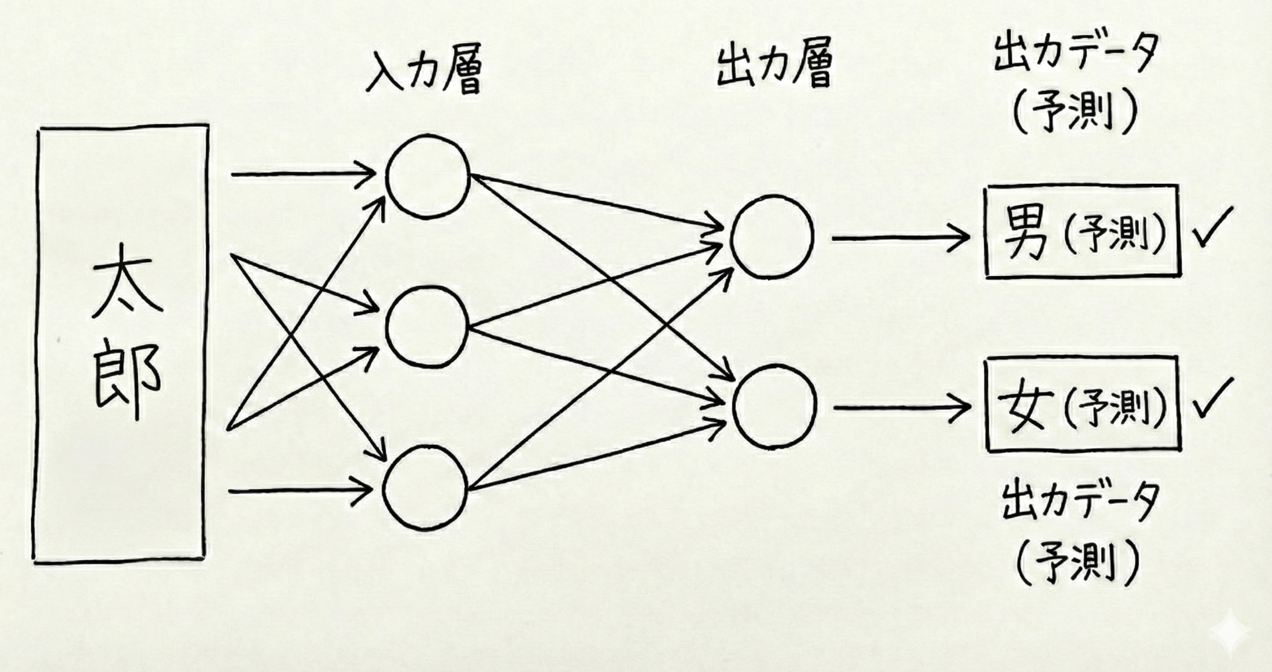
\includegraphics[width=.76\textwidth]{class13/nnimage.png}\end{center}

\section{今日の内容}
1.

文章のベクトル化

2.

パーセプトロンのモデルと構築
                    名前から男/女を判定するモデル

3.

ニューラルネットの数学的モデル

4.

研究の内容と今後の展開

\section{アルファベットの数字化}
\section{ルール}
A → 1,　B → 2,　C → 3,　...　Z → 26

\section{例}
\paragraph{例}
CAT

→

(3, 1, 20)


\paragraph{例}
DOG

→

(4, 15, 7)


\paragraph{例}
HELLO

→

( ?, ?, ?, ?, ? )


📝 自分の下の名前をベクトルで表せ

\section{アルファベット → 数字 対応表}
A\allowbreak{} 1

B\allowbreak{} 2

C\allowbreak{} 3

D\allowbreak{} 4

E\allowbreak{} 5

F\allowbreak{} 6

G\allowbreak{} 7

H\allowbreak{} 8

I\allowbreak{} 9

J\allowbreak{} 10

K\allowbreak{} 11

L\allowbreak{} 12

M\allowbreak{} 13

N\allowbreak{} 14

O\allowbreak{} 15

P\allowbreak{} 16

Q\allowbreak{} 17

R\allowbreak{} 18

S\allowbreak{} 19

T\allowbreak{} 20

U\allowbreak{} 21

V\allowbreak{} 22

W\allowbreak{} 23

X\allowbreak{} 24

Y\allowbreak{} 25

Z\allowbreak{} 26

\paragraph{例}
CAT

→

(3, 1, 20)


\paragraph{例}
HARUTO

→

(8, 1, 18, 21, 20, 15)


\section{文章のベクトル化}
文章にでてくるそれぞれの単語をベクトル化し、\allowbreak{} 0をはさんで結合して新しいベクトルを作る。

\section{例}
\paragraph{例}
I AM CAT

→

\( (9) + (1, 13) + (3, 1, 20) \)

=

\( (9, 0, 1, 13, 0, 3, 1, 20) \)


\paragraph{例}
YOU ARE DOG

→

( ?, ?, ... )


文章の集合

Vect
→

ベクトルの集合

\section{二進数化}
コンピュータでは 0と1 の方が扱いやすい。\allowbreak{} 
（変換された時のビット数は5で統一する）

\section{変換例}
26
\(= 2^4 + 2^3 + 2^1\)
→
11010

10
\(= 2^3 + 2^1\)
→
01010

3
\(= 2^1 + 2^0\)
→
00011

1
\(= 2^0\)
→
00001

数の集合

Bin
→

\( \{0, 1\}^5 \)

\section{数字→二進数}
各数字を 5ビット の二進数に変換

\begin{center}
\begin{tabularx}{\textwidth}{|>{\raggedright\arraybackslash}X|>{\raggedright\arraybackslash}X|}\hline
数値 & 二進数 \\ \hline
1 & 00001 \\ \hline
2 & 00010 \\ \hline
3 & 00011 \\ \hline
4 & 00100 \\ \hline
5 & 00101 \\ \hline
6 & 00110 \\ \hline
7 & 00111 \\ \hline
8 & 01000 \\ \hline
9 & 01001 \\ \hline
\end{tabularx}
\end{center}

\begin{center}
\begin{tabularx}{\textwidth}{|>{\raggedright\arraybackslash}X|>{\raggedright\arraybackslash}X|}\hline
数値 & 二進数 \\ \hline
10 & 01010 \\ \hline
11 & 01011 \\ \hline
12 & 01100 \\ \hline
13 & 01101 \\ \hline
14 & 01110 \\ \hline
15 & 01111 \\ \hline
16 & 10000 \\ \hline
17 & 10001 \\ \hline
18 & 10010 \\ \hline
\end{tabularx}
\end{center}

\begin{center}
\begin{tabularx}{\textwidth}{|>{\raggedright\arraybackslash}X|>{\raggedright\arraybackslash}X|}\hline
数値 & 二進数 \\ \hline
19 & 10011 \\ \hline
20 & 10100 \\ \hline
21 & 10101 \\ \hline
22 & 10110 \\ \hline
23 & 10111 \\ \hline
24 & 11000 \\ \hline
25 & 11001 \\ \hline
26 & 11010 \\ \hline
0 & 00000 \\ \hline
\end{tabularx}
\end{center}

A〜Z, 空白

Bin
→

\( \{0, 1\}^5 \)

\section{文章の二進数化}
N文字の文章

→

\( BV = \mathrm{Bin} \circ \mathrm{Vect} \)

→

\( \{0, 1\}^{5N} \)

※ 空白（スペース）は 00000 に変換する

\section{例}
\paragraph{例}
I AM CAT
→
\( (9, 0, 1, 13, 0, 3, 1, 20) \)

→
\( (0,1,0,0,1, \underbrace{0,0,0,0,0}_{\text{空白}}, 0,0,0,0,1, 0,1,1,0,1, \underbrace{0,0,0,0,0}_{\text{空白}}, 0,0,0,1,1, 0,0,0,0,1, 1,0,1,0,0) \)


\section{名前の二進数化}
名前を 5ビット × 10文字 = 50ビット のベクトルに変換する

★ 名前が10文字未満のときは，\allowbreak{} 
最初に 00000 を必要な個数だけ加えて 50ビットにそろえる

名前

→

Binary

→

\( \{0,1\}^{50} \)

\section{例}
SHUTA（5文字）\allowbreak{} 
        ↓\allowbreak{} 

        \( \underbrace{00000\cdots00000}_{\text{最初に5文字分}}
        \;10011\,01000\,10101\,10100\,00001 \)

📝 自分の名前を 50ビットにせよ

\section{名前から男/女判定}
10文字の下の名前が200個与えられているとする。\allowbreak{} 
        それぞれの名前には男/女が分かっている。

\section{例}
SHUTA
→
男 = 1

TAKASHI
→
男 = 1

REIKA
→
女 = 0

名前をBinaryで表すと...

\( \mathbf{x} \in \Sigma \mapsto y_{\mathbf{x}} \in \{0, 1\} \)

\section{パーセプトロンのモデル}
\subsection{📐 設定}
\( \Sigma = \{\mathbf{x}_1, \ldots, \mathbf{x}_M\} \) : M個の名前（二進数化されたもの）の集合\allowbreak{} 
                \( \mathbf{x}_i \in \{0, 1\}^{50} \) : 10文字の名前の二進数化\allowbreak{} 
                \( \mathbf{1} = (1, 1, \ldots, 1) \) : 50次元のベクトル\allowbreak{} 
                \( 2\mathbf{x} - \mathbf{1} = (2x_1 - 1, \ldots, 2x_{50} - 1) \in \{-1, 1\}^{50} \)

x₁

x₂

...

x₇₅

Σ

→

0 or 1

\emph{目標: 次を満たす} \( \mathbf{w} = (w_1, \ldots, w_{50}) \in \{-1, 1\}^{50} \) を見つける\allowbreak{} 
\( \mathbf{1}\{ \mathbf{w} \cdot (2\mathbf{x} - \mathbf{1}) \ge 0 \} = y_{\mathbf{x}} \)　　∀ \( \mathbf{x} \in \Sigma \)

\section{判定の仕組み}
\( \mathbf{w} \) として \( \mathbf{1}\{ \mathbf{w} \cdot (2\mathbf{x} - \mathbf{1}) \ge 0 \} = y_{\mathbf{x}} \)　∀ \( \mathbf{x} \in \Sigma \)を満たすものが取れたとする。

データにない新しい名前 x' が来た時の判定方法:

新しい名前\allowbreak{} YUKI

→

二進数化\allowbreak{} \( \mathbf{x}' \)

→

内積計算\allowbreak{} \( \mathbf{w} \cdot (2\mathbf{x}' - \mathbf{1}) \)

→

判定結果

1

\( \mathbf{w} \cdot (2\mathbf{x}' - \mathbf{1}) \) を計算する

2

結果が \( \ge 0 \) なら 1（男）

3

結果が \( < 0 \) なら 0（女）

\paragraph{補足}
💡 学習で見つけた

\emph{w}

を使って、未知のデータを分類できる！


\section{実装}
📊

\subsection{データ}
JSON形式で1000件以上収集

\begin{verbatim}
[
  {"name": "HARUTO", "sex": 1},
  {"name": "SAKURA", "sex": 0},
  {"name": "YUKI", "sex": 1},
  {"name": "HINATA", "sex": 0},
  ...
]
\end{verbatim}

sex: 1=男, 0=女

🤖

\subsection{モデル}
パーセプトロンを実装\allowbreak{} 
\emph{w} はモンテカルロで探索\allowbreak{} \allowbreak{} 
精度：約87\%

\# モンテカルロの概要\allowbreak{} 
for t = 1, 2, ..., T:\allowbreak{} 
                w' ← wの1成分をランダムに反転\allowbreak{} 
                if E(w') ≤ E(w):　\# 誤分類が減ったら採用\allowbreak{} 
                    w ← w'\allowbreak{} 
\# E(w) = 誤分類の数（モデルが間違えた予測の個数）

\section{デモ：名前から性別を予測 🔮}
日本人の名前をローマ字で入力してください（例：HARUTO、SAKURA）\allowbreak{} 
        ニューラルネットワークで学習したモデルが性別を予測します（精度：約87\%）

\emph{学習された重みベクトル \( \mathbf{w} \in \mathbb{R}^{50} \)：}

\allowbreak{}

w = [-5.07, -5.07, -5.07, -5.07, -5.07, 76.05, 116.22, 138.04, -180.43, 59.57, -5.07, -5.07, -5.07, -5.07, -5.07, 38.61, 24.25, -4.79, -41.25, -1.37, -5.07, -5.07, -5.07, -5.07, -5.07, 8.61, 1.66, 2.64, -16.63, 0.55, -5.07, -5.07, -5.07, -5.07, -5.07, 16.94, -10.08, 5.41, 17.13, -7.50, -5.07, -5.07, -5.07, -5.07, -5.07, 11.30, -2.92, 8.30, 11.18, 11.10, -5.07, -5.07, -5.07, -5.07, -5.07, 16.82, -11.84, 5.16, 23.58, -35.49, -5.07, -5.07, -5.07, -5.07, -5.07, -10.82, -40.59, -27.64, -31.87, -6.35, -5.07, -5.07, -5.07, -5.07, -5.07, -29.47, -2.93, 30.79, -35.59, 59.11]

※ 10文字 × 5bit = 50次元。

\paragraph{補足}
💡 試してみよう：YUKI、HARUKA、TSUBASA など中性的な名前はどう判定される？


\section{一般のパーセプトロンのモデル}
\subsection{📐 設定}
\( N, M \) を固定する\allowbreak{} 
                \( \Sigma = (\mathbf{x}^1, \mathbf{x}^2, \ldots, \mathbf{x}^M) \subset \{-1, 1\}^N \) : 入力データ\allowbreak{} 
                各 \( \mathbf{x} \in \Sigma \) に対し、\( y_{\mathbf{x}} \in \{-1, 1\} \) : ラベル

\( \mathbf{x} \in \{-1, 1\}^N \)\allowbreak{} 
入力

×

\( \mathbf{w} \in \{-1, 1\}^N \)\allowbreak{} 
重み

→

\( y \in \{-1, 1\} \)\allowbreak{} 
出力

\emph{解の存在:} 次を満たす \( \mathbf{w} = (w_1, \ldots, w_N) \in \{-1, 1\}^N \) が存在するとき\allowbreak{} 
\( \mathbf{1}\{ \mathbf{w} \cdot \mathbf{x} \ge 0 \} = y_{\mathbf{x}} \)　　∀ \( \mathbf{x} \in \Sigma \)\allowbreak{} 
            モデルは「解をもつ」という\allowbreak{} 
※ \( \mathbf{w} \) を見つける問題は\emph{NP困難}

\section{ニューラルネットの確率モデル}
ニューラルネットは、出力が複数個あるようなパーセプトロン

\begin{figuretext}
x₁ \quad x₂ \quad ... \quad xₙ \quad 入力 \quad y₁ \quad y₂ \quad y₃ \quad 出力 \quad W \quad N × K 行列
\end{figuretext}

\section{例：名前から複数属性を判定}
SHUTA

→

男
関東
50代以下

→

\( (1, 1, 0) \)

TAKASHI

→

男
関西
50代以上

→

\( (1, 0, 1) \)

REIKA

→

女
関東
??

→

\( (0, 1, \, ??) \)

\section{ニューラルネットの確率モデル}
確率論では入力と出力が独立な確率変数で与えられる場合を考える

\subsection{📐 設定}
\( (\mathbf{x}^1, \mathbf{y}^1), (\mathbf{x}^2, \mathbf{y}^2), \ldots, (\mathbf{x}^M, \mathbf{y}^M) \in \{-1, 1\}^N \times \{-1, 1\}^K \)\allowbreak{} 
\( \mathbf{x}^i \in \{-1,1\}^N \)、\( \mathbf{y}^i \in \{0,1\}^K \) を一様・独立に選ぶ

重み行列

\[ \mathbf{W} = \begin{pmatrix} w_{11} & w_{12} & \cdots & w_{1K} \\ w_{21} & w_{22} & \cdots & w_{2K} \\ \vdots & \vdots & \ddots & \vdots \\ w_{N1} & w_{N2} & \cdots & w_{NK} \end{pmatrix}  \in \{-1, 1\}^{N \times K} \]

\emph{解の存在:} 次を満たす行列 \( \mathbf{W} \) が存在するとき\allowbreak{} 
\( \mathbf{1}\{ \mathbf{W}\mathbf{x}^i \ge 0 \} = \mathbf{y}^i \)　　∀ \( i = 1, \ldots, M \)\allowbreak{} 
            ニューラルネットは「解をもつ」という

\section{解の個数の定義}
\subsection{📐 パラメータ設定}
\( \alpha, \beta > 0 \) を固定する\allowbreak{} 
                \( M = \alpha N \)（データ数）、\( K = \beta N \)（出力次元）\allowbreak{} 
                \( \mathbf{x}^i \in \{-1,1\}^N \)、\( \mathbf{y}^i \in \{0,1\}^K \) を 一様・独立 に選ぶ

\emph{解の個数:}\allowbreak{} 
\[ Z_{N,M,K} = \#\left\{ \mathbf{W} \in \{-1, 1\}^{N \times K} : \mathbf{1}\{ \mathbf{W}\mathbf{x}^i \ge 0 \} = \mathbf{y}^i, \; \forall i \right\} \]

\( \alpha < \alpha_c \)

\( Z_{N,M,K} > 0 \) w.h.p.

✓

\( \alpha_c \)

\( \alpha > \alpha_c \)

\( Z_{N,M,K} = 0 \) w.h.p.

✗

\( \alpha \)（データ数 / 次元）→

\paragraph{補足}
💡 データが多すぎると（\( \alpha > \alpha_c \)）、すべてを正しく分類する重み \( \mathbf{W} \) は存在しなくなる！


\section{研究の歴史}
🔬

\subsubsection{モデルの起源（20世紀中盤）}
McCulloch–Pitts '43, Rosenblatt '58, Gardner '85 など\allowbreak{} 
                    パーセプトロンは単層ニューラルネットとして知られる

🎲

\subsubsection{Gardner (1985)}
レプリカトリックを用いて \( \displaystyle\lim_{N\to \infty} \frac{\log{Z_{N,\alpha N}}}{N} \) を計算：
                    \[ \mathbb{E}[\log{Z}]=\lim_{n\to 0} n^{-1} (\mathbb{E}[Z^n]-1) \]
                    これが「Gardner 公式」の由来

📜

\subsubsection{Talagrand (1998)}
\( \alpha \ll 1 \) の場合に Gardner 公式を数学的に証明

❓

\subsubsection{未解決問題}
\( \alpha \) が小さくない場合の問題は未解決

\section{RS公式}
\subsection{📐 RS公式（Ising Perceptron）}
\[
                    f_{\mathrm{RS}}(\alpha)
                    = \inf_{q \in [0,1]} \sup_{r \ge 0}
                    \Big\{
                        -\frac{r}{2}\log(1-q)
                        + \alpha \, \mathbb{E}\Big[\log \mathbb{P}\Big(Z_2\geq \sqrt{\tfrac{q}{1-q}}\,Z_1\Big|~Z_1\Big)\Big]
                        + \mathbb{E}\big[\log 2\cosh(\sqrt{r}\,Z_1)\big]
                    \Big\}
                \]

ここで \(Z_1, Z_2\) は独立な標準正規分布に従う確率変数

\emph{臨界値の定義:}\allowbreak{} 
\[ \alpha_c^* = \sup\{\alpha > 0 : f_{\mathrm{RS}}(\alpha) > 0\} \]

\paragraph{補足}
💡 RS = Replica Symmetric（レプリカ対称性）

\allowbreak{}

統計物理のレプリカ法から導かれる公式


\section{予想：解の数の漸近挙動}
\paragraph{予想}
\subsection{予想：解の数の漸近挙動}
\(\alpha < \alpha_c^*\) のとき：
                \[ \lim_{N \to \infty} (KN)^{-1} \log Z_{N, \alpha N,K} = f_{\mathrm{RS}}(\alpha) \]

\(\alpha > \alpha_c^*\) のとき：
                \[ \mathbb{P}(Z_{N, \alpha N} = 0) \to 1 \]

解の数の対数が RS 公式で正確に計算できる（と予想される）


\paragraph{補足}
💡 この予想が正しければ、臨界値 \(\alpha_c^*\) で

シャープな相転移

が起こる


\section{Talagrandの定理}
\subsection{定理 (Talagrand 1998)}
M. Talagrand (1998)

\( \alpha \ll 1 \)

（十分小さい \( \alpha \)）に対して、

\[ \lim_{N \to \infty} N^{-2} \log Z_{N, \alpha N,\beta N} = \beta f_{\mathrm{RS}}(\alpha) \]

が成り立つ。

\paragraph{補足}
💡 これは RS 公式が

数学的に正しい

ことを示した初めての結果！

\allowbreak{}

しかし、\( \alpha \) が小さい場合に限られる。


\( \alpha \ll 1 \)

Talagrand ✓

未解決領域

Open Problem

\section{\(\alpha_{N,K}\) の定義}
\subsection{定義}
入力：

\(\mathbb{R}^N\)

出力：

\(K\)

クラス（\(\{1,\dots,K\}\)）

\allowbreak{}

\(Z_{N,M,K}\)

：\(M\) 個のデータをすべて同時に満たす「解の個数」。

\allowbreak{}

臨界点を次で定義する。

\[
                \alpha_{N,K} := \max\left\{ \frac{M}{N} \;\middle|\; Z_{N,M,K} \ge 1 \right\}
                \]

\paragraph{補足}
💡

意味：

データ密度 \(\alpha = M/N\) を増やしていき、

\emph{まだ解が少なくとも1つ存在する最大の値}

。

\allowbreak{}


\section{臨界点集中定理}
\subsection{定理 (Nakajima-Sun 2024)}
S. Nakajima \& N. Sun (2024)

ある数列

\( (\alpha_c^*(N))_{N\in \mathbb{N}} \)

が存在して、 任意の \( \delta > 0 \) に対して、

\[ \mathbb{P}\left( \left| \alpha_{N,\beta N} - \alpha_c^*(N) \right| > \delta \right) \to 0, \quad N\to \infty\]

✓

臨界値の存在

→

?

極限の計算\allowbreak{} \( \alpha_c^*(N) \to \alpha_c^* \)

→

...

深層学習への拡張

\paragraph{補足}
💡 臨界値 \( \alpha_c^*(N) \) が存在することは証明された。次のステップは \( N \to \infty \) での極限！

\allowbreak{}

※ \( K = 1 \) の場合は Xu (2021) が同じ定理を証明


\section{さらなる展開}
🧠

\subsubsection{深層学習への拡張}
複数の隠れ層を持つネットワークの場合はどうなるか？

\begin{figuretext}
入力 \quad 隠れ層1 \quad 隠れ層2 \quad 隠れ層3 \quad 出力 \quad ?
\end{figuretext}

\section{多層パーセプトロン（MLP）}
パーセプトロンを 層として積み重ねたもの。$\ell$層の長さを$N_\ell\in \mathbb N$と置く。

\begin{figuretext}
入力 \( g \) \quad 層 1 \quad 層 2 \quad 出力 \( \hat y \) \quad 重み \( W^{(1)}, W^{(2)}, \dots \)
\end{figuretext}

\subsection{定義}
入力 \(h^{(0)}=g \in \{-1,1\}^N\)と重み$W_\ell\in \{-1,1\}^{N_\ell \times N_{\ell-1}}$に対し，
      \[h^{(\ell)}={\rm sgn}\!\left(W^{(\ell)} h^{(\ell-1)}\right),\quad \ell=1,\dots,L,\]
      \[\hat y={\rm sgn}\!\left(W^{(L+1)} h^{(L)}\right).\]

\section{多層パーセプトロンの学習問題}
\section{データ}
\(N=\sum_{\ell=1}^{L} N_{\ell}N_{\ell+1}\)とおく。\allowbreak{} 
        \( M \) 個の入力とラベル\allowbreak{} 
        \[(g^i, y^i),\ i=1,\dots,M.\]
        典型的に \( M=\alpha N \)（データ数は次元に比例）。

\paragraph{補足}
💡 このスライド以降では

\allowbreak{}

入力 \( g^i \) とラベル \( y^i \) は独立に\( \{-1,1\}^{N_1\times N_{L+1}} \)上の一様測度から選ぶ。


\section{予測}
入力\allowbreak{} \( g^i \)

→

MLP\allowbreak{} \( W^{(1)},\dots,W^{(L+1)} \)

→

出力\allowbreak{} \( \hat y^i \)

目標：全ての \( i \) で
        \( \hat y^i = y^i \)
        を満たす重みを見つける。

\section{解の個数と相転移}
\subsection{解の個数（深さ \( L \)）}
重みを \( \{-1,1\} \) に制限して（離散化して）数える：
      \[Z_{N,M}^{(L)}=\#\Bigl\{(W^{(1)},\dots,W^{(L+1)}) : \hat y^i=y^i,\ \forall i\Bigr\}.\]
      深さや中間層幅の取り方で \( Z_{N,M}^{(L)} \) の典型挙動が変わる。

$\alpha < \alpha_c^{(L)}$

$Z_{N,\alpha N}^{(L)} > 0$ が起こりやすい

✓

$\alpha_c^{(L)}$

$\alpha > \alpha_c^{(L)}$

$Z_{N,\alpha N}^{(L)} = 0$ が起こりやすい

✗

$\alpha = M/N$（データ密度）→

\section{最終的な予想（ランダムMLP）}
\paragraph{予想}
\subsection{予想：自由エネルギーの極限と臨界点}
深さ $L$ を固定し，$M=\alpha N$ とする。\allowbreak{} \allowbreak{} 
      データ $(g^i,y^i)_{i=1}^{M}$ は
      独立に \( \{-1,1\}^{N_1\times N_{L+1}} \)の一様測度から選ぶ。\allowbreak{} \allowbreak{} 

      このとき，ある定数関数 \( f^{(L)}(\alpha) \) が存在して
      \[\frac{1}{N}\log Z_{N,\alpha N}^{(L)} \ \to\ f^{(L)}(\alpha)\quad \text{in probability},\]
      さらに
      \[\alpha_c^{(L)}=\sup\{\alpha>0:\ f^{(L)}(\alpha)>0\}\]
      でシャープな相転移が起こる。


\paragraph{補足}
💡 ポイント：ここでは

\( g \) と \( y \) を一様 \( \{-1,1\} \)

に取るモデル。 深さ \( L \) や活性化 \( \varphi \) の違いが \( \alpha_c^{(L)} \) をどう動かすかが中心問題。


🙏

\section{ご清聴ありがとうございました}
中島 秀太 / Shuta Nakajima\allowbreak{} 
慶應義塾大学


\fi
\backmatter
\end{document}
